\chapter{Foundations for inference}
\label{foundationsForInference}
\label{ch_foundations_for_inf}
\renewcommand{\chapterfolder}{ch_foundations_for_inf}

Statistical inference is concerned primarily with understanding the
accuracy of parameter estimates. While the equations and details change
depending on the setting, the foundations for inference are the same
throughout all of statistics.
\begin{enumerate}
\item[\ref{pointEstimates}] We start with a familiar topic:
    the notion of using a sample proportion as our estimate
    of a population proportion. Our goal in this section
    is to understand that estimate's variability from one
    sample to the next.
\item[\ref{confidenceIntervals}] Next, rather than providing
    a single point estimate, we create what's called a
    \hiddenterm{confidence interval}, which is a range
    of values where the population value is likely to lie.
\item[\ref{hypothesisTesting}] In the third section,
    we introduce a hypothesis testing framework, which allows
    us to formally evaluate claims about the population,
    such as \emph{"a survey shows a candidate has a majority
    of support"} of the voting population.
\item[\ref{aFrameworkForInference}] Lastly, we touch on how
    the methods in this chapter generalize to many other
    situations. While the details may vary from one
    application to another, the core methods are the same.
\end{enumerate}

%What you learn in this chapter will be applied in many contexts.

%Each of the ideas in this chapter are applicable to a broad set of
%applications and new contexts. We'll expand on these ideas in later
%chapters.

\Comment{Do additional checks to confirm that the term
\emph{standard error} is being used consistently rather than
\emph{standard deviation}.}

\Comment{Planning to aggressively cut out the usage of
    ``true'', as in ``true proportion'', in OS4.}





%__________________
\section{Point estimates and sampling variability}
\label{pointEstimates}

\index{data!solar survey|(}

\newcommand{\pewsolarpollsize}{1000}
\newcommand{\pewsolarpollprop}{0.887}
\newcommand{\pewsolarpollpropcomplement}{0.113}
\newcommand{\pewsolarpollpercent}{88.7}
\newcommand{\pewsolarpollpercentcomplement}{11.3}
\newcommand{\pewsolarpollcount}{887}
\newcommand{\pewsolarpollcountcomplement}{113}
\newcommand{\pewsolarpollse}{0.0100}

Pew Research conducted a poll of 1000
American adults' support of different forms of energy.
They found that \pewsolarpollpercent{}\% of respondents
favored expanding
solar energy.\footnote{The full survey's sample size was 2541,
and we've taken a subsample. To find the survey details, see\\
\oiRedirect{textbook-pew_2018_poll_on_solar_and_wind_expansion}{www.pewinternet.org/2018/05/14/majorities-see-government-efforts-to-protect-the-environment-as-insufficient}}
A~natural question is,
\Comment{The redirect link in the footnote needs to be confirmed as
working.}
\begin{quote}
If the poll was based on only thousand people, how reliable is it?
\end{quote}
If we took another poll, we wouldn't get the exact same answer.
Maybe we'd get 90\%, or perhaps even 80\%.
Ultimately, it's unlikely that the actual proportion of Americans
who support expanding solar energy is \emph{exactly}
\pewsolarpollpercent{}\%, but the data suggests the actual
support is close to \pewsolarpollpercent{}\%.

In this section, we discuss what a point estimate like
\pewsolarpollpercent{}\% represents
and the uncertainty associated with such an estimate. We'll also
use some new notation and terminology:
\begin{itemize}
\item The population proportion will be written as $p$.
    When discussing a population summary such as $p$,
    it is common to refer to the value as a population
    \term{parameter}.
    In the solar survey,
    $p$ represents the proportion of \emph{all}
    American adults who support solar energy.
\item Using Pew Research sample, we can estimate that the proportion
    of American adults who support expanding solar energy is
    somewhere near \pewsolarpollpercent{}\%.
    This is called the \term{sample proportion},
    and it gets a special label of $\hat{p}$
    (spoken as \emph{p-hat}).
\item The size of a sample will generally
    be denoted by $n$. In the case of this Pew Research poll,
    the \term{sample size} is $n = \pewsolarpollsize{}$.
\end{itemize}

\subsection{Point estimates and error}

\index{point estimate|(}

A sample proportion $\hat{p}$ is called
the \term{point estimate} of the parameter $p$, since based
on the sample, this is our single best estimate of $p$.

The Pew Research poll is a point estimate
of the actual proportion
of American adults that support expanding solar energy.
This estimate of \pewsolarpollpercent{}\% is unlikely
to be perfect,
and it's quite possible for the population proportion
to be a little lower or a little higher than the
sample proportion.
The difference between a point estimate and
the parameter is called the estimate's \term{error}.

The error varies from one sample to the next: maybe
in one sample it is 1\% too low while in another
it is 3\% too high. Unfortunately, we rarely know the direction
or size of the error in our estimates, so instead we focus
on understanding what kinds of errors are typical.


\subsection{Understanding the variability of a point estimate}
\label{simulationForUnderstandingVariabilitySection}

We want to understand \emph{how does the
sample proportion $\hat{p}$ behave when the population
proportion is about \pewsolarpollprop{}}. We could
run the survey again to see how consistent the results
are, but who has the time and money for that? Instead,
we can investigate the properties of $\hat{p}$ using simulations.

To simulate the sample, we'll suppose that the population
proportion is exactly \pewsolarpollpercent{}\%.
%Now, we know
%the population proportion isn't exactly \pewsolarpollpercent\%,
%but we do expect it to be close, so this simulation will offer
%us some insights about the property of $\hat{p}$.
%If we took a random sample
%from this population, how accurate would the point estimate be?
Here's how we might simulate it:
\begin{enumerate}
\item There were about 250 million American adults in 2018.
    On 250 million pieces of paper, write ``support''
    on \pewsolarpollpercent{}\% of them and ``not'' on
    the other \pewsolarpollpercentcomplement{}\%.
\item Mix up the pieces of paper and pull out \pewsolarpollsize{}
    pieces to represent our sample of 1000 American adults.
\item Compute the fraction of the sample that say ``support''.
\end{enumerate}
Any volunteers to conduct this simulation? Probably not. Running
this simulation with 250 million pieces of paper would be
time-consuming and very costly, but we can simulate it
using computer code; we've written a short program in
Figure~\ref{solarPollSimulationCodeR}.
In this simulation, the sample gave a point estimate of
$\hat{p}_1 = 0.901$. We~know the population proportion
for the simulation was $p = \pewsolarpollprop{}$, so we know
the estimate had an error of +0.014.

%\setlength\textwidth{\officialtextwidth-10mm}
\begin{figure}
\texttt{\# 1.\ Create a set of 250 million entries,
where 89\% of them are "support" \\
\#\ \ \ \ and 11\% are "not". \\
possible\_entries <- rep(c("support", "not"),
    c(\pewsolarpollprop{}, \pewsolarpollpropcomplement{}) * 250e6)\\
\# 2.\ Sample \pewsolarpollsize{} of the entries. \\
sampled\_entries <- sample(possible\_entries, \pewsolarpollsize{}) \\
\# 3.\ Count the number that are "justified", then divide
by the sample size. \\
sum(sampled\_entries == "justified") / \pewsolarpollsize{}}
\caption{Code for a simulation using the
    statistical software called \R\index{R}.
    Each line that starts with \texttt{\#} is a \term{code comment},
    which is used to describe in regular language what the
    code is doing.}
\label{solarPollSimulationCodeR}
\end{figure}
% \setlength\textwidth{\officialtextwidth}

One simulation isn't enough to get a great sense of the
distribution of estimates we might expect in the simulation,
so we should run more simulations.
In a second simulation,
we get $\hat{p}_2 = 0.892$, which has an error of~+0.005.
In another, $\hat{p}_3 = 0.885$ for an error of -0.002. And in another,
an estimate of $\hat{p}_4 = 0.866$ with an error of -0.021.
With the help of a computer, we've run the simulation 10,000 times
and created a histogram of the results from all 10,000 simulations
in Figure~\ref{sampling_10k_prop_887p}. This
distribution of sample proportions is called a
\term{sampling distribution}.
We can characterize this sampling distribution as follows:
\begin{description}
\item[Center.] The center of the distribution is
    $\bar{x}_{\hat{p}} = \pewsolarpollprop{}0$, which is the same as the
    population proportion.
    That~is, we see that the sample proportion is an
    \termsub{unbiased estimate}{unbiased}
    of the population proportion.
\item[Spread.] The standard deviation of the distribution
    is $s_{\hat{p}} = \pewsolarpollse{}$. When we're talking about
    a sampling distribution or the variability of
    a point estimate, we typically use the term
    \termsub{standard error}{standard error (SE)}
    rather than \emph{standard deviation},
    and the notation $SE_{\hat{p}}$ is used for the standard
    error associated with the sample proportion.
\item[Shape.] The distribution is symmetric and bell-shaped,
    and it \emph{resembles a normal distribution}.
\end{description}
These findings are very encouraging! When the population
proportion is $p = \pewsolarpollprop{}$ and the sample size is
$n = \pewsolarpollsize{}$,
the sample proportion $\hat{p}$ tends to give a pretty good estimate
of the population proportion. We also have this interesting observation
that the histogram resembles a normal distribution.

\begin{figure}
   \centering
   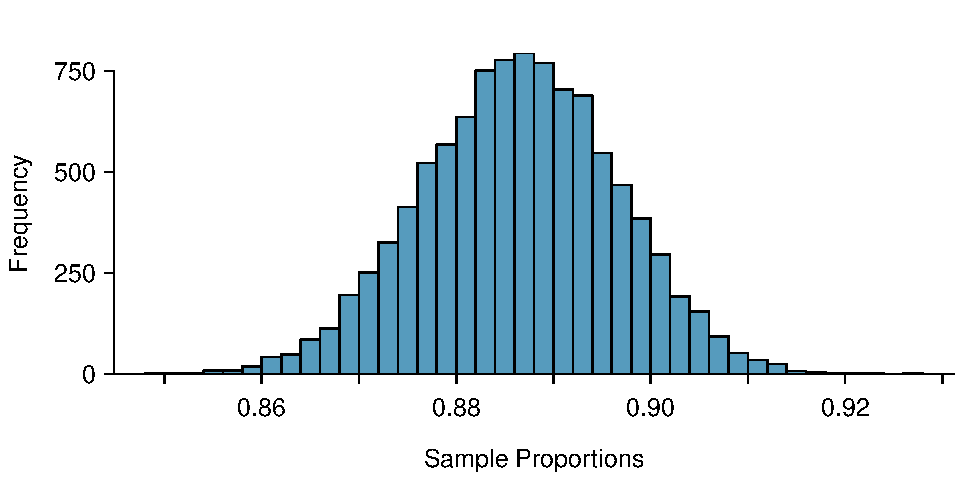
\includegraphics[width=0.8\textwidth]{ch_foundations_for_inf/figures/sampling_10k_prop_887p/sampling_10k_prop_887p}
   \caption{A histogram of 10,000 sample proportions, where each
       sample is taken from a population where the population
       proportion is \pewsolarpollprop{} and the sample size is
       $n = \pewsolarpollsize{}$.}
   \label{sampling_10k_prop_887p}
\end{figure}

\begin{onebox}{Sampling distributions are
    never observed, but we keep them in mind}
  In real-world applications, we never actually observe the
  sampling distribution, yet it is useful to always think of
  the sample proportion as coming from such a distribution.
  Understanding the sampling distribution will help us
  characterize and make sense of the individual point
  estimate that we do observe.
\end{onebox}

\begin{examplewrap}
\begin{nexample}{If we used a much smaller sample size of $n = 50$,
would you guess that the standard error for $\hat{p}$ would be larger
or smaller than when we used $n = \pewsolarpollsize{}$?}
\label{smallerSampleWhatHappensToPropErrorExercise}
Intuitively, it seems like more data is better
than less data, and generally that is correct! The typical error
when $p = \pewsolarpollprop{}$ and $n = 50$ would be larger
than the error we would expect when $n = \pewsolarpollsize{}$.
\end{nexample}
\end{examplewrap}

%\noindent
Example~\ref{smallerSampleWhatHappensToPropErrorExercise}
highlights an important property: a bigger sample
tends to provide a more precise point estimates than a smaller sample.

\index{point estimate|)}


\subsection{Central Limit Theorem}

The distribution in
Figure~\ref{sampling_10k_prop_887p} looks an awful lot like
a normal distribution. That is no anomaly; it~is the result
of a general principle called the \term{Central Limit Theorem}.
\index{Central Limit Theorem!proportion|textbf}

\begin{onebox}{Central Limit Theorem and the success-failure condition}
  When observations are independent and the sample size is
  sufficiently large, the sample proportion $\hat{p}$ will tend
  to follow a normal distribution with the following mean and
  standard error:
  \begin{align*}
    \mu_{\hat{p}} &= p
    &SE_{\hat{p}} &= \sqrt{\frac{p (1 - p)}{n}}
  \end{align*}
  The sample size is typically considered sufficiently large when
  $np \geq 10$ and $n(1-p) \geq 10$, which is called the
  \term{success-failure condition}.
\end{onebox}

The Central Limit Theorem is incredibly important, and it provides
a foundation for much of statistics. As we begin applying
this principle, be mindful of the two requirements:
the observations must be independent, and the the sample size must
be sufficiently large such that $np \geq 10$ and $n(1-p) \geq 10$.

\begin{examplewrap}
\begin{nexample}{Earlier we estimated the mean and standard
error of the $\hat{p}$'s using simulated data when
$p = \pewsolarpollprop{}$ and $n = \pewsolarpollsize{}$.
Confirm that the Central Limit Theorem applies and the sampling 
distribution is approximately normal.}\label{sample_p887_n1000_confirm_normal}
\begin{description}
\item[Independence.] There are $n = \pewsolarpollsize{}$
    observations for each
    sample proportion $\hat{p}$, and each of those observations
    are independent draws. \emph{The most common way for
    observations to be considered independent is if they are from
    a simple random sample.}
    \index{independent}
    \index{independence}
    \index{Central Limit Theorem!independence}
\item[Success-failure condition.] We can confirm the sample size
    is sufficiently large by checking the success-failure condition
    and confirming the two calculated values are greater than~10:
    \begin{align*}
    np &= \pewsolarpollsize{} \times \pewsolarpollprop{}
        = \pewsolarpollcount{}
        \geq 10
    &n(1-p) &= \pewsolarpollsize{} \times (1 - \pewsolarpollprop{})
        = \pewsolarpollcountcomplement{}
        \geq 10
    \end{align*}
\end{description}
The independence and success-failure conditions are both 
satisfied, so the Central Limit Theorem applies and we can assume 
that the sampling distribution follows the normal distribution.
\end{nexample}
\end{examplewrap}

\begin{onebox}{How to verify sample observations are independent}
  Subjects in an experiment are considered independent
  if they undergo random assignment to the treatment
  groups.\vspace{3mm}

  If the observations are from a simple random sample that is sampled 
  without replacement and consist of fewer than 10\% of the population, 
  then they are independent.
  Even if the sample is bigger than 10\%, assuming independence
  will lead to more conservative results.\vspace{3mm}

  If a sample is from a seemingly random process,
  e.g. an occasional error on an assembly line,
  checking independence is more difficult. In~this case,
  use your best judgement.
\end{onebox}

\begin{examplewrap}
\begin{nexample}{Compute the theoretical mean and standard error
of the $\hat{p}$'s when
$p = \pewsolarpollprop{}$ and $n = \pewsolarpollsize{}$,
according to the
Central Limit Theorem.}\label{sample_p887_n1000_mean_se}
The mean of the $\hat{p}$'s is simply the population proportion:
$\mu_{\hat{p}} = \pewsolarpollprop{}$.

The calculation of the standard error of $\hat{p}$ uses
the following formula:
\begin{align*}
SE_{\hat{p}}
    = \sqrt{\frac{p (1 - p)}{n}}
    = \sqrt{\frac{\pewsolarpollprop{} (1 - \pewsolarpollprop{})}{1000}}
    = \pewsolarpollse{}
\end{align*}
\end{nexample}
\end{examplewrap}

\begin{examplewrap}
\begin{nexample}{Estimate how frequently the sample proportion
$\hat{p}$ should be within 0.02 (2\%) of the population value,
$p = \pewsolarpollprop{}$. Based on
Examples~\ref{sample_p887_n1000_confirm_normal}
and~\ref{sample_p887_n1000_mean_se}, we know that the distribution is
$N(\mu_{\hat{p}} = \pewsolarpollprop{}, SE_{\hat{p}} = \pewsolarpollse{})$.}
\label{sampling_10k_prop_887p-prop_from_867_to_907}
After so much practice in Section~\ref{normalDist},
this normal distribution example will hopefully feel familiar!
We would like to understand the fraction of $\hat{p}$'s
between 0.867 and 0.907:
\begin{center}
\includegraphics[width=60mm]{ch_foundations_for_inf/figures/p-hat_from_867_and_907/p-hat_from_867_and_907}
\end{center}
With $\mu_{\hat{p}} = \pewsolarpollprop{}$ and
$SE_{\hat{p}} = \pewsolarpollse{}$,
we can compute the Z-score for both the left and right cutoffs:
\begin{align*}
Z_{0.867} &= \frac{0.867 - \pewsolarpollprop{}}{\pewsolarpollse{}} = -2
&Z_{0.907} &= \frac{0.907 - \pewsolarpollprop{}}{\pewsolarpollse{}} = 2
\end{align*}
We can use either statistical software, a graphing calculator,
or a table to find the areas to the tails, and in any case we
will find that they are each 0.0228. The total tail areas are
$2 \times 0.0228 = 0.0456$, which leaves the shaded area of
0.9544. That is, about 95.44\% of the sampling distribution
in Figure~\ref{sampling_10k_prop_887p} is within $\pm0.02$
of the simulation population proportion, $p = \pewsolarpollprop{}$.
\end{nexample}
\end{examplewrap}

\begin{exercisewrap}
\begin{nexercise}
In Example~\ref{smallerSampleWhatHappensToPropErrorExercise}
we discussed how a smaller sample would tend
to produce a less reliable estimate. Explain how this intuition
is reflected in the formula for
$SE_{\hat{p}} = \sqrt{\frac{p (1 - p)}{n}}$.\footnotemark
\end{nexercise}
\end{exercisewrap}
\footnotetext{Since the
    sample size $n$ is in the denominator of the fraction (on the
    bottom of the fraction), a bigger sample size means the entire
    expression when calculated will tend to be smaller. That is,
    a larger sample size would correspond to a smaller standard
    error.}


\subsection{Applying the Central Limit Theorem to a real-world setting}

Think back to the 2018 poll where
$\hat{p} = \pewsolarpollprop{}$ of American adults favored
expanding solar energy. We might wonder: does the sample
proportion from the poll approximately follow a normal
distribution?
We check the conditions from the Central Limit Theorem:
\begin{description}
\item[Independence.] The poll is a simple random sample of
    American adults, which means that the observations are
    independent.
\item[Success-failure condition.] To check this condition,
    we need the population proportion, $p$, to check if both
    $np$ and $n(1-p)$ are greater than 10. However, we do not
    know the value of $p$; that's exactly why the pollsters
    took a sample! In cases like these, we often use $\hat{p}$
    as our next best way to check the success-failure condition:
    \begin{align*}
    n\hat{p} &= \pewsolarpollsize{} \times \pewsolarpollprop{}
        = \pewsolarpollcount{}
    &n (1 - \hat{p}) &= \pewsolarpollsize{} \times (1 - \pewsolarpollprop{})
        = \pewsolarpollcountcomplement{}
    \end{align*}
    While we cannot check the condition with $p$,
    the sample proportion $\hat{p}$ acts as
    a reasonable substitute, and each value is comfortably
    above the minimums of 10.
\end{description}

This \term{substitution approximation} of using $\hat{p}$ in
place of $p$ will also be useful when computing the standard error
of the sample proportion in many situations:
\begin{align*}
SE_{\hat{p}}
    = \sqrt{\frac{p (1 - p)}{n}}
    \approx \sqrt{\frac{\hat{p} (1 - \hat{p})}{n}}
    = \sqrt{\frac{\pewsolarpollprop{}
        (1 - \pewsolarpollprop{})}{\pewsolarpollsize{}}}
    = \pewsolarpollse{}
\end{align*}
This substitution approximation technique is useful in many
situations.


\subsection[Better understanding the Central Limit Theorem
    (special~topic)]
  {Better understanding the Central Limit Theorem \\
      \mbox{(special~topic)}}



We've applied the Central Limit Theorem in numerous examples
so far this chapter:
\begin{quote}{\em
When observations are independent and the sample size is
sufficiently large, the distribution of $\hat{p}$ resembles
a normal distribution with
\begin{align*}
  \mu_{\hat{p}} &= p
  &SE_{\hat{p}} &= \sqrt{\frac{p (1 - p)}{n}}
\end{align*}
The sample size is considered sufficiently large
when $n p \geq 10$ and $n (1 - p) \geq 10$.
}\end{quote}
In this section, we'll explore the success-failure
condition and seek to better understand the
Central Limit Theorem.

An easier question to answer is, \emph{what happens when
$np < 10$ or $n(1-p) < 10$?} As we did in
Section~\ref{simulationForUnderstandingVariabilitySection},
we can simulate drawing samples of different sizes where,
say, $p = 0.25$. Here's a sample of
size~10:
\begin{center}
% paste(sample(c("yes", "no"), 10, TRUE, c(.25, .75)), collapse = ", ")
no, no, yes, yes, no, no, no, no, no, no
\end{center}
In this sample, we observe a sample proportion of yeses
of $\hat{p} = \frac{2}{10} = 0.2$. We can simulate many such
proportions to understand the sampling distribution of
$\hat{p}$ when $n = 10$ and $p = 0.25$, which we've plotted
in Figure~\ref{sampling_10_prop_25p}
alongside a normal distribution with the
same mean and standard deviation. These distributions
look nothing alike.

\begin{figure}[t]
   \centering
   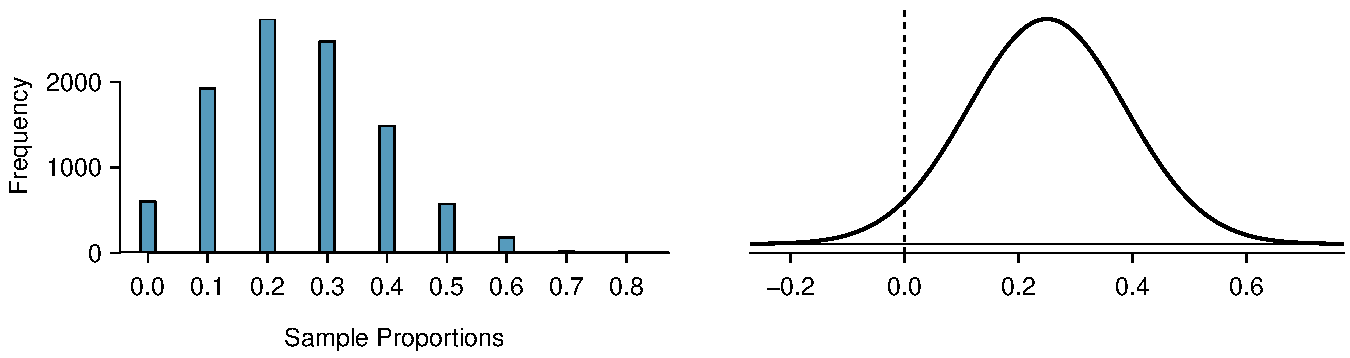
\includegraphics[width=0.97\textwidth]{ch_foundations_for_inf/figures/sampling_10_prop_25p/sampling_10_prop_25p}
   \caption{Left: simulations of $\hat{p}$ when the sample size
       is $n = 10$ and the population proportion is $p = 0.25$.
       Right: a normal distribution with the same mean (0.25)
       and standard deviation (0.137).}
   \label{sampling_10_prop_25p}
\end{figure}

\begin{figure}
   \centering
   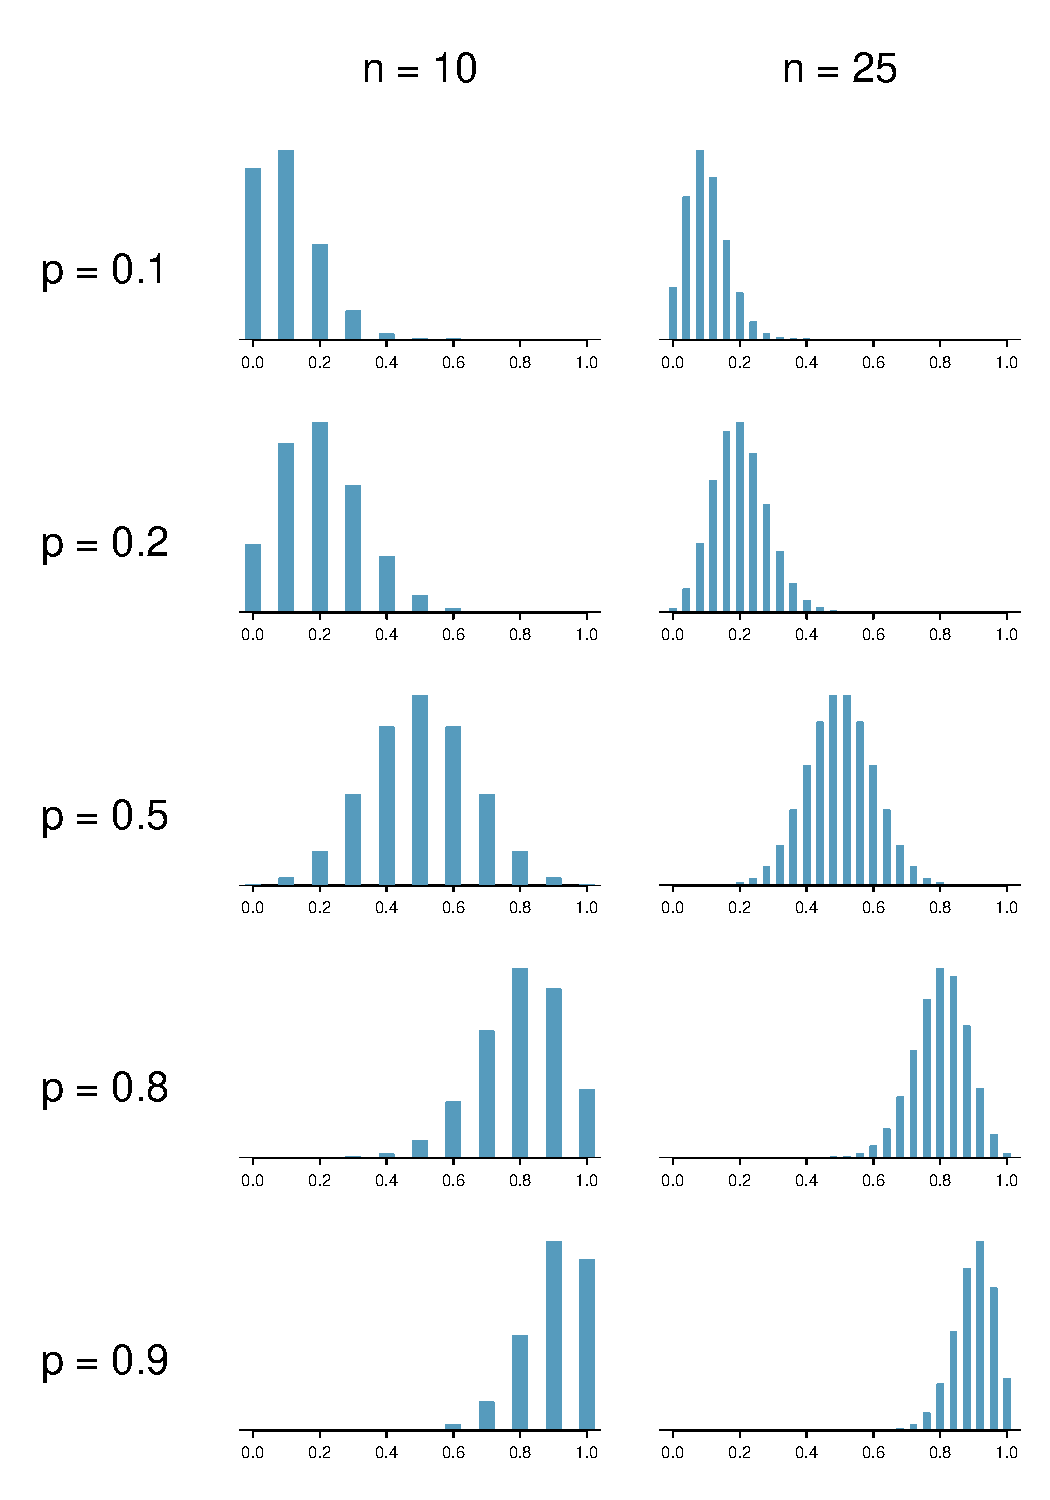
\includegraphics[width=\textwidth]{ch_foundations_for_inf/figures/clt_prop_grid/clt_prop_grid_1}
   \caption{Sampling distributions for several scenarios
       of $p$ and $n$. \\ \ }
   \label{clt_prop_grid_1}
\end{figure}

\begin{figure}
   \centering
   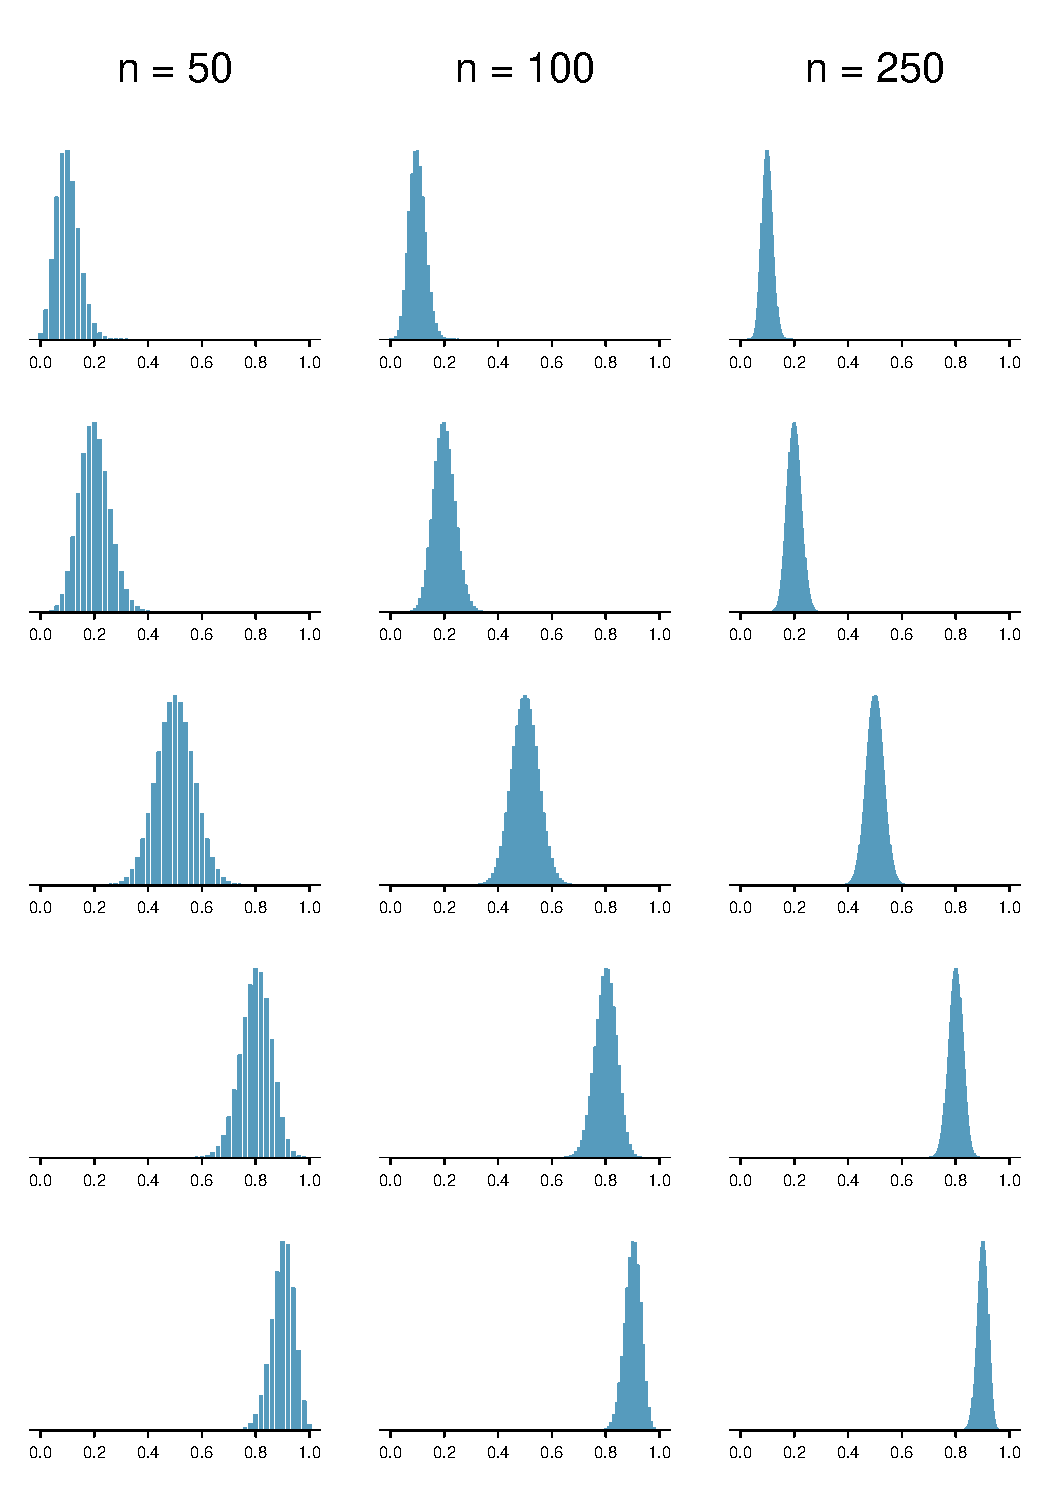
\includegraphics[width=\textwidth]{ch_foundations_for_inf/figures/clt_prop_grid/clt_prop_grid_2}
   \caption{Sampling distributions for several scenarios
       of $p$ and $n$. \\
       Rows: $p = 0.10$, $p = 0.20$, $p = 0.50$,
       $p = 0.80$, and $p = 0.90$.}
   \label{clt_prop_grid_2}
\end{figure}

\begin{center}
\begin{tabular}{lccc}
\hline
    &  Unimodal?  &  Smooth?  &  Symmetric? \\
\hline
Normal  &  \highlightO{Yes}  &  \highlightO{Yes}  &
    \highlightO{Yes} \\
$n = 10$, $p = 0.25$  &  \highlightO{Yes}  &
    \highlightT{No}  &  \highlightT{No} \\
\hline
\end{tabular}
\end{center}
Notice that the success-failure condition
was not satisfied when $n = 10$ and $p = 0.25$:
\begin{align*}
n p = 10 \times 0.25 = 2.5 &&
    n (1 - p) = 10 \times 0.75 = 7.5
\end{align*}
This single sampling distribution does not show that
the success-failure condition is the perfect guideline,
but we have found that the guideline did correctly
identify that the normal distribution was not appropriate.

\pagebreak

\Comment{Used an artificial page break here to make the
    transition smoother. Delete this comment when doing
    final formatting.}

\Comment{Ensure the two full-page figures are on pages
    facing each other for the print version.}

We can complete several additional simulations,
shown in
Figures~\ref{clt_prop_grid_1}
and~\ref{clt_prop_grid_2}.
We can see some trends:
\begin{enumerate}
\item When either $np$ or $n(1 - p)$ is small, the
    distribution is more \term{discrete},
    i.e. \emph{not continuous}.
\item When $np$ or $n(1-p)$ is smaller than~10,
    the skew in the distribution is more noteworthy.
\item The larger both $np$ \emph{and} $n(1 - p)$,
    the more normal the distribution.
    This may be a little harder to see for the larger
    sample size in these plots as the variability
    also becomes much smaller.
\item When $np$ and $n(1 - p)$ are both very large,
    the distribution's discreteness is hardly evident,
    and the distribution looks much more
    like a normal distribution.
\end{enumerate}

So far we've only focused on the skew and discreteness
of the distributions. We haven't considered
how the mean and standard error
of the distributions change.
Take a moment to look back at the graphs,
and pay attention to three things:
\begin{enumerate}
\item The centers of the distribution are always at
    the population proportion, $p$, that was used to
    generate the simulation. Because the sampling
    distribution of $\hat{p}$ is always centered at
    the population parameter $p$, it means the sample
    proportion $\hat{p}$ is \term{unbiased} when
    the data are independent and drawn from such
    a population.
\item For a particular population proportion $p$,
    the variability in the sampling distribution
    decreases as the sample size~$n$ becomes larger.
    This will likely align with your intuition:
    an estimate based on a larger sample size will
    tend to be more accurate.
\item For a particular sample size, the variability
    will be largest when $p = 0.5$. The differences
    may be a little subtle, so take a close look.
    This reflects the importances of the proportion
    $p$ in the standard error formula:
    $SE = \sqrt{\frac{p (1 - p)}{n}}$.
    The standard error is largest when $p = 0.5$.
\end{enumerate}

At no point will the distribution of $\hat{p}$ look
\emph{perfectly} normal.
It is always a matter of degree, and we will use
the standard success-failure condition with minimums
of 10 for $np$ and $n (1 - p)$ as our guideline
within this~book.




%__________________
\section{Confidence intervals for a sample proportion}
\label{confidenceIntervals}

\index{confidence interval|(}

The sample proportion $\hat{p}$ provides a single plausible value
for the population proportion $p$. However, the sample proportion
isn't perfect and will have some \emph{standard error}
associated with it. When stating an estimate for the population 
proportion, it is better practice to provide a plausible 
\emph{range of values} instead of supplying just the point estimate.

\subsection{Capturing the population parameter}

Using only a point estimate is like fishing in a murky
lake with a spear. We can throw a spear where we
saw a fish, but we will probably miss. On the other hand,
if we toss a net in that area, we have a good chance of
catching the fish.
A \term{confidence interval} is like fishing with a net,
and it represents a range of plausible values where we
are likely to find the population parameter.

If we report a point estimate $\hat{p}$, we probably
will not hit the exact population proportion. On the
other hand, if we report a range of plausible values,
representing a confidence interval,
we have a good shot at capturing the parameter.

\begin{exercisewrap}
\begin{nexercise}
If we want to be very certain we capture the population
proportion in an interval, should we use a wider interval
or a smaller interval?\footnotemark
\end{nexercise}
\end{exercisewrap}
\footnotetext{If we want to be more
    certain we will capture the fish, we might use a
    wider net. Likewise, we use a wider confidence interval
    if we want to be more certain that we capture the
    parameter.}

\subsection{An approximate 95\% confidence interval}

Our sample proportion $\hat{p}$ is the most plausible
value of the population proportion, so it makes sense
to build a confidence interval around this point estimate.
The \hiddenterm{standard error} provides a guide for how
large we should make the confidence interval.

The standard error represents the standard deviation
of the point estimate, and when the Central
Limit Theorem conditions are satisfied, we also know
that the point estimate closely follows a normal
distribution. In a normal distribution, about 95\% of
the data is within 2 standard deviations of the mean.
Using this principle, we can construct a confidence
interval that extends 2 standard errors from the sample
proportion to be \term{95\% confident}\index{confident|textbf}
that the interval captures the population proportion:
\begin{align*}
\text{point estimate}\ &\pm\ 2\times SE \\
\hat{p}\ &\pm\ 2\times SE_{\hat{p}}
%\label{95PercentConfidenceIntervalFormula}
\end{align*}
But what does ``95\% confident'' mean? Suppose we took
many samples and built a 95\% confidence interval from
each sample. Then about 95\% of those intervals would
contain the parameter, $p$.
Figure~\ref{95PercentConfidenceInterval} shows this
process with 25 samples from the simulation in
Section~\ref{simulationForUnderstandingVariabilitySection},
where 24 of the resulting confidence intervals contain
the simulation's population proportion of
$p = \pewsolarpollprop{}$, and one interval does not.

\begin{figure}
   \centering
   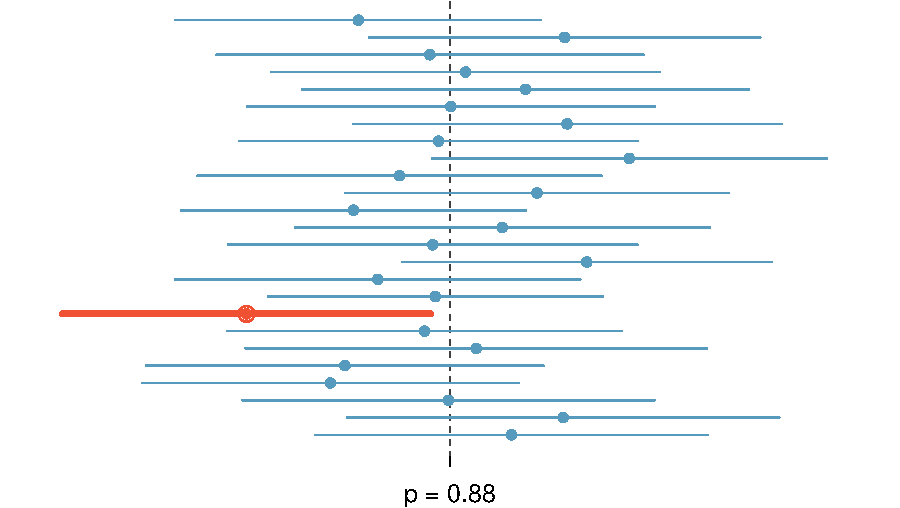
\includegraphics[width=0.75\textwidth]{ch_foundations_for_inf/figures/95PercentConfidenceInterval/95PercentConfidenceInterval}
   \caption{Twenty-five point estimates and confidence
       intervals from the simulations in
       Section~\ref{simulationForUnderstandingVariabilitySection}.
       For~each sample, a 95\% confidence interval was
       constructed and shown relative to the population
       proportion $p = \pewsolarpollprop{}$. Only~1 of these~25
       intervals did not capture the population
       proportion.}
   \label{95PercentConfidenceInterval}
\end{figure}

\begin{examplewrap}
\begin{nexample}{In Figure~\ref{95PercentConfidenceInterval},
one interval does not contain $p = \pewsolarpollprop{}$.
Does this imply that the population proportion cannot be
$p = \pewsolarpollprop{}$?}
Just as some observations occur more than 2 standard deviations
from the mean, some point estimates will be more than
2 standard errors from the parameter of interest.
A confidence interval only provides a plausible range
of values. While we might say other values are implausible
based on the data, this does not mean they are impossible.
\end{nexample}
\end{examplewrap}

While about 95\% of the data is within 2 standard deviations
in a normal distribution, it would be more precise to use
a value of 1.96 standard deviations. This more precise value
is typically what is used to construct a
95\% confidence interval.

\begin{onebox}{95\% confidence interval for a parameter}
  \index{confidence interval!95\%}
  When a point estimate qualifies for the Central Limit
  Theorem and closely follows a normal distribution,
  we can construct a 95\% confidence interval as
  \begin{align*}
  \text{point estimate} &\pm 1.96 \times SE
  \end{align*}
\end{onebox}

\begin{examplewrap}
\begin{nexample}{In Section~\ref{pointEstimates} we learned about
    a poll where \pewsolarpollpercent{}\% of a random sample of
    \pewsolarpollsize{} American adults
    supported expanding the role of solar power. Compute and
    interpret a 95\% confidence interval for the population
    proportion.} \label{95p_ci_for_pew_solar_support}
  We earlier confirmed that $\hat{p}$ follows a normal
  distribution and has a standard error of
  $SE_{\hat{p}} = \pewsolarpollse{}$.
  To compute the 95\% confidence interval, plug the
  point estimate $\hat{p} = \pewsolarpollprop{}$ and
  standard error into the 95\% confidence interval formula:
  \begin{align*}
  \hat{p} \pm 1.96 \times SE_{\hat{p}}
  \quad\to\quad
  \pewsolarpollprop{} \pm 1.96 \times \pewsolarpollse{}
  \quad\to\quad
  (0.8674, 0.9066)
  \end{align*}
  We are 95\% confident that the actual proportion of
  American adults who support expanding solar power is
  between 86.74\% and 90.66\%.
\end{nexample}
\end{examplewrap}


\subsection{Changing the confidence level}
\label{changingTheConfidenceLevelSection}

\index{confidence interval!confidence level|(}

Suppose we want to consider confidence intervals where the confidence
level is higher than 95\%, such as a confidence
level of~99\%. Think back to the analogy about trying to catch a fish:
if~we want to be more sure that we will catch the fish, we should use
a wider net. To create a 99\% confidence level, we must also widen our
95\% interval. On the other hand, if we want an interval with lower
confidence, such as 90\%, we could use a slightly narrower interval than
our original 95\% interval.

The 95\% confidence interval structure provides guidance in how to
make intervals with new confidence levels. The general 95\% confidence
interval for a point estimate that follows the normal distribution is
\begin{eqnarray*}
\text{point estimate}\ \pm\ 1.96\times SE
\end{eqnarray*}
There are three components to this interval: the point estimate,
``1.96'', and the standard error. The choice of $1.96\times SE$ was
based on capturing 95\% of the data since the estimate is within
1.96 standard errors of the parameter about 95\% of the time.
The choice of 1.96 corresponds to a 95\% confidence level. 

\begin{exercisewrap}
\begin{nexercise} \label{leadInForMakingA99PercentCIExercise}
If $X$ is a normally distributed random variable, how often will $X$
be within 2.58 standard deviations of the mean?\footnotemark
\end{nexercise}
\end{exercisewrap}
\footnotetext{This is equivalent to asking how often the
    Z-score will be larger than -2.58 but less than 2.58.
    For a picture, see Figure~\ref{choosingZForCI}.
    To determine this probability, we can use statistical software,
    a calculator, or a table to look up -2.58 and 2.58 for
    the normal distribution: 0.0049 and 0.9951.
    Thus, there is a $0.9951-0.0049 \approx 0.99$ probability
    that an unobserved normal random variable
    $X$ will be within 2.58 standard deviations of $\mu$.}

Guided Practice~\ref{leadInForMakingA99PercentCIExercise} highlights
that 99\% of the time a normal random variable will be within
2.58 standard deviations of the mean.
To create a 99\% confidence interval, change 1.96 in the 95\%
confidence interval formula to be $2.58$.
That is, the formula
for a 99\% confidence interval is
\begin{align*}
\text{point estimate}\ \pm\ 2.58\times SE
%\label{99PercCIForProp}
\end{align*}

\begin{figure}
  \centering
  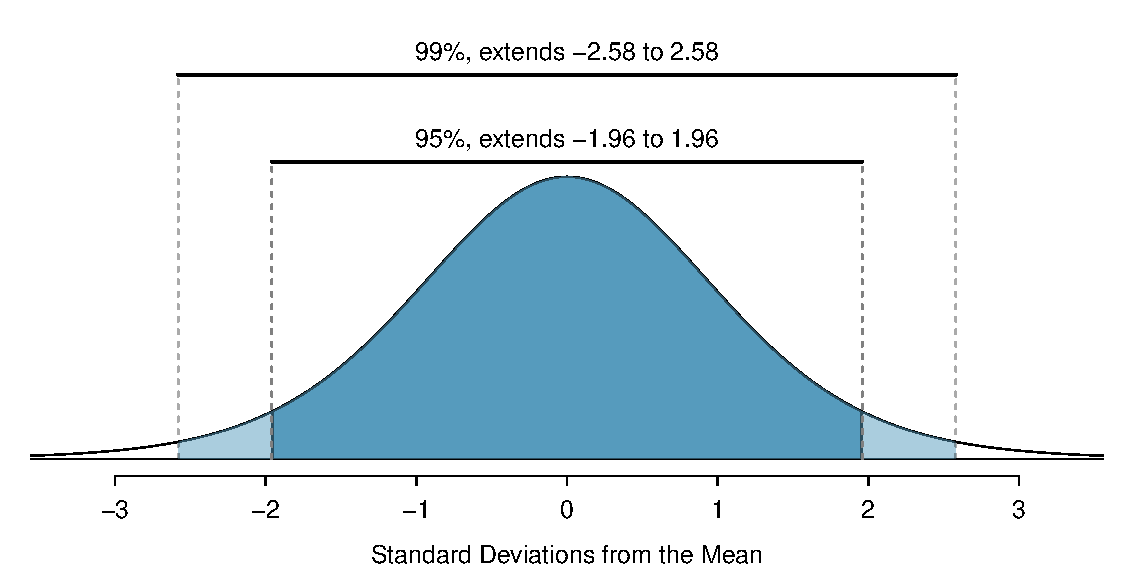
\includegraphics[width=\textwidth]{ch_foundations_for_inf/figures/choosingZForCI/choosingZForCI}
  \caption{The area between -$z^{\star}$ and $z^{\star}$ increases as
      $z^{\star}$ becomes larger. If the confidence level is 99\%,
      we choose $z^{\star}$ such that 99\% of the normal curve is
      between -$z^{\star}$ and $z^{\star}$, which corresponds to 0.5\%
      in the lower tail and 0.5\% in the upper tail: $z^{\star}=2.58$.}
\label{choosingZForCI}
\index{confidence interval!confidence level|)}
\end{figure}

This approach -- using the Z-scores in the
normal model to compute confidence levels --
is appropriate when a point estimate such as $\hat{p}$
is associated with a normal distribution.
%For the context of sample proportions, the
%normal distribution is reasonable when the sample
%observations are independent and the success-failure condition
%holds ($np$ and $n(1-p)$ are both at least 10).
For some other point estimates, the normal model is not a good fit;
in these cases, we'll use alternative distributions that better
represent the sampling distribution.

\begin{onebox}{Confidence interval using any confidence level}
  If a point estimate closely follows the normal model
  with standard error $SE$, then a confidence interval
  for the population parameter is
  \begin{align*}
  \text{point estimate}\ \pm\ z^{\star} SE
  \end{align*}
  where $z^{\star}$ corresponds to the confidence
  level selected.
\end{onebox}

Figure~\ref{choosingZForCI} provides a picture of how to identify
$z^{\star}$ based on a confidence level. We~select $z^{\star}$
so that the area between -$z^{\star}$ and $z^{\star}$ in the normal
distribution corresponds to the confidence level. 

\begin{onebox}{Margin of error}
  \label{marginOfErrorTermBox}%
  In a confidence interval, $z^{\star}\times SE$ is called the
  \term{margin of error}.
\end{onebox}

\begin{examplewrap}
\begin{nexample}{Use the data in
    Example~\ref{95p_ci_for_pew_solar_support} to
    create a 90\% confidence interval for the proportion of American
    adults that support expanding solar power students.
    We have already verified conditions for normality.}
  We first find $z^{\star}$ such that 90\% of the distribution falls
  between -$z^{\star}$ and $z^{\star}$ in the standard normal model,
  $N(\mu=0, \sigma=1)$. We can do this using a graphing calculator,
  statistical software, or a probability table by looking for an upper
  tail of 5\% (the other 5\% is in the lower tail): $z^{\star}=1.65$.
  The 90\% confidence interval can then be computed as
  \begin{align*}
  \hat{p}\ \pm\ 1.65\times SE_{\hat{p}}
      \quad\to\quad 0.887\ \pm\ 1.65\times 0.0100
      \quad\to\quad (0.8705, 0.9035)
  \end{align*}
  That is, we are 90\% confident that 87.1\% to 90.4\% of American
  adults supported the expansion of solar power in 2018.
\end{nexample}
\end{examplewrap}



\subsection{More case studies}

\index{data!Ebola poll|(}

\newcommand{\wsjebolapollsize}{1042}
\newcommand{\wsjebolapollsizecomma}{1,042}
\newcommand{\wsjebolapollprop}{0.82}
\newcommand{\wsjebolapollpropcomplement}{0.18}
\newcommand{\wsjebolapollpercent}{82}
\newcommand{\wsjebolapollpercentcomplement}{18}
\newcommand{\wsjebolapollcount}{854}
\newcommand{\wsjebolapollcountcomplement}{188}
\newcommand{\wsjebolapollse}{0.012}


In New York City on October 23rd, 2014, a doctor who had recently been
treating Ebola patients in Guinea went to the hospital with a slight fever
and was subsequently diagnosed with Ebola. Soon thereafter,
an NBC~4 New York/The Wall Street Journal/Marist Poll found that
\wsjebolapollpercent{}\% of New Yorkers favored a ``mandatory 21-day
quarantine for anyone who has come in contact with an Ebola
patient''.\footnote{\oiRedirect{textbook-maristpoll_ebola_201410}{Poll
ID NY141026 on maristpoll.marist.edu}.} This poll included responses
of \wsjebolapollsizecomma{} New York adults between
Oct 26th and~28th, 2014.
%We may want a confidence interval for the proportion of New York
%adults who favored a mandatory quarantine of anyone who had been in
%contact with an Ebola patient.

\begin{examplewrap}
\begin{nexample}{What is the point estimate in this case,
    and is it reasonable to
    use the normal distribution to model that point estimate?}
  The point estimate, based on a sample of size $n = \wsjebolapollsize{}$,
  is $\hat{p} = \wsjebolapollprop{}$. To check whether $\hat{p}$ can be reasonably
  modeled using the normal distribution, we check independence
  (the poll is based on a simple random sample) and the
  success-failure condition
  ($\wsjebolapollsize{} \times \hat{p} \approx \wsjebolapollcount{}$
  and $\wsjebolapollsize{} \times (1 - \hat{p})
      \approx \wsjebolapollcountcomplement{}$,
  both easily greater than~10). With the conditions met, we are assured
  that the sampling distribution of $\hat{p}$ can be modeled using
  a normal distribution.
\end{nexample}
\end{examplewrap}

\begin{examplewrap}
\begin{nexample}{Estimate the standard error of
    $\hat{p} = \wsjebolapollprop{}$ from the Ebola survey.}
  We'll use the substitution approximation of
  $p \approx \hat{p} = \wsjebolapollprop{}$ to compute the standard error:
  \begin{align*}
  SE = \sqrt{\frac{p(1-p)}{n}}
    \approx \sqrt{\frac{\wsjebolapollprop{}
        (1 - \wsjebolapollprop{})}{\wsjebolapollsize{}}}
    = \wsjebolapollse{}
  \end{align*}
\end{nexample}
\end{examplewrap}

\begin{examplewrap}
\begin{nexample}{Construct a 95\% confidence interval for $p$,
    the proportion of New York adults who supported a quarantine
    for anyone who has come into contact with an Ebola patient.}
  Using the standard error $SE = 0.012$ from
  Example~\ref{seOfPropOfAmericansJobApprovalOfSupremeCourt},
  the point estimate \wsjebolapollprop{}, and $z^{\star} = 1.96$
  for a 95\% confidence level, the confidence interval is
  \begin{eqnarray*}
  \text{point estimate} \ \pm\ z^{\star}SE
    \quad\to\quad \wsjebolapollprop{} \ \pm\ 1.96\times \wsjebolapollse{}
    \quad\to\quad (0.796, 0.844)
  \end{eqnarray*}
  We are 95\% confident that the proportion of New York adults
  in October 2014 who supported a quarantine for anyone who had come
  into contact with an Ebola patient was between 0.796 and 0.844.
\index{data!Ebola poll|)}
\end{nexample}
\end{examplewrap}

\begin{exercisewrap}
\begin{nexercise}
Do you think the confidence interval is still valid for the opinions
of New Yorkers today?\footnotemark
\end{nexercise}
\end{exercisewrap}
\footnotetext{Not necessarily. The poll was taken at a
time where there was a huge public safety concern. Now that people
have had some time to step back, they may have changed their opinions.
We would need to run a new poll if we wanted to get an estimate of the
current proportion of New York adults who would support such a
quarantine period.}

\index{data!wind turbine survey|(}

\newcommand{\pewwindpollsize}{\pewsolarpollsize}
\newcommand{\pewwindpollprop}{0.848}
\newcommand{\pewwindpollpropcomplement}{0.152}
\newcommand{\pewwindpollpercent}{84.8}
\newcommand{\pewwindpollpercentcomplement}{15.2}
\newcommand{\pewwindpollcount}{848}
\newcommand{\pewwindpollcountcomplement}{152}
\newcommand{\pewwindpollse}{0.0114}

In the poll by Pew Research asking about solar energy, the
researchers also inquired about other forms of energy.
In this next case study, we examine the support for expanding wind
turbines, which received support from \pewwindpollpercent{}\%
of the \pewwindpollsize{} respondents.

\begin{exercisewrap}
\begin{nexercise}\label{pew_wind_turbine_support_normal_dist_gp}
Is the normal approximation reasonable in this case?\footnotemark
\end{nexercise}
\end{exercisewrap}
\footnotetext{We
check independence, which is okay since this survey was a simple
random sample, and also the success-failure condition
($\pewwindpollsize{} \times \pewwindpollprop{} = \pewwindpollcount{}$
and $\pewwindpollsize{} \times \pewwindpollpropcomplement{}
    = \pewwindpollcountcomplement$ are both at least 10).
Since both conditions are satisfied,
$\hat{p} = \pewwindpollprop{}$ can be
modeled using the normal distribution.}

\begin{exercisewrap}
\begin{nexercise}
Using the Pew Research survey where $n = \pewwindpollsize{}$ and
$\hat{p} = \pewwindpollprop{}$, create a 99\% confidence interval
for the level of American support for expanding the use of wind
turbines for power
generation.\footnotemark
\end{nexercise}
\end{exercisewrap}
\footnotetext{Guided
Practice~\ref{pew_wind_turbine_support_normal_dist_gp}
confirmed that that $\hat{p}$ closely follows a normal distribution,
so we can use the confidence interval formula:
\begin{align*}
\text{point estimate} \pm z^{\star} SE
\end{align*}
In this case, the point estimate is $\hat{p} = \pewwindpollprop{}$.
For a 99\% confidence interval, $z^{\star} = 2.58$. Computing the
standard error:
$SE_{\hat{p}}
  = \sqrt{\frac{\pewwindpollprop{}(1 - \pewwindpollprop{})}
      {\pewwindpollsize{}}}
  = \pewwindpollse{}$.
Finally, we compute the interval as
$\pewwindpollprop{} \pm 2.58 \times \pewwindpollse{} \to (0.8186, 0.8774)$.
It is also important to \emph{always} provide an interpretation
for the interval: we are 99\% confident the proportion of
American adults that support expanding the use of wind
turbines is between 81.9\% and 87.7\% in 2018.}


\subsection{Interpreting confidence intervals}
\label{interpretingCIs}

\index{confidence interval!interpretation|(}

In each of the examples, we described the confidence
intervals by putting them into the context of the data and also
using somewhat formal language:
\begin{description}
  \item[Solar.] We are 90\% confident that 87.1\% to 90.4\% of
      American adults support the expansion of solar power in 2018.
  \item[Ebola.] We are 95\% confident that the proportion
      of New York adults in October 2014 who supported a quarantine
      for anyone who had come into contact with an Ebola patient was
      between 0.796 and 0.844.
  \item[Wind Turbine.] We are 99\% confident the proportion of
      Americans adults that support expanding the use of wind
      turbines is between 81.9\% and 87.7\% in 2018.
\end{description}
First, notice that the statements are always about the population
parameter, which considers \emph{all} American adults for the
energy polls and \emph{all} New York adults for the quarantine poll.

We also avoided another common mistake:
\emph{incorrect} language might try to describe the confidence interval
as capturing the population parameter with a certain probability.
Making a probability interpretation is a common error:
while it might be useful to think of it as a probability,
the confidence level only quantifies how plausible
it is that the parameter is in the given interval.

Another important consideration of confidence intervals is that they
\emph{only try to capture the population parameter}. A confidence
interval says nothing about the confidence of capturing individual
observations, a proportion of the observations, or about capturing
point estimates. Confidence intervals only attempt to capture
population parameters.

\index{data!wind turbine survey|)}
\index{data!solar survey|)}
\index{confidence interval!interpretation|)}

\CalculatorVideos{confidence intervals for a single proportion}

\index{confidence interval|)}




%__________________
\section{Hypothesis testing for a proportion}
\label{hypothesisTesting}

\index{hypothesis testing|(}

The following question comes from Hans Rosling's book
\emph{\oiRedirect{amazon_factfulness}{Factfulness}}:
\begin{quote}{\em
  In the last 20 years the proportion of the
  world population living in extreme poverty has:
  \begin{enumerate}[a.]
  \item Almost doubled.
  \item More or less stayed the same.
  \item Almost halved.
  \end{enumerate}
}\end{quote}
Write down what your answer (or guess),
and when you're ready, find the answer in the
footnote.\footnote{The correct answer is (c):
extreme poverty has been nearly cut in half in the last 20~years.}

In this section,
we'll be exploring how people with a 4-year college
degree perform on this and other world health questions.

\newcommand{\roslingAsize}{50}
\newcommand{\roslingAprop}{0.24}
\newcommand{\roslingApropcomplement}{0.76}
\newcommand{\roslingApercent}{24}
\newcommand{\roslingApercentcomplement}{76}
\newcommand{\roslingAcount}{12}
\newcommand{\roslingAcountcomplement}{38}
\newcommand{\roslingAse}{0.060}
% n <- 50; x <- 12; (p <- x/n); (se <- sqrt(p * (1 - p) / n)); p + c(-1, 1) * 1.96 * se

%There's an adage in United States financial markets that
%it is better to get out of investments during the six ``summer''
%months: \emph{sell in May and go away!}\footnote{Summer in the
%northern hemisphere, anyways. \rotatebox[origin=c]{180}{(Hello
%Australia!)}} While this clever saying does rhyme, that doesn't
%mean it is sound financial advice. Let's investigate.

%so is this is a pretty strong statement, since the stock
%market has a very strong historical trend of moving upwards.
%
%To test this theory, we've retrieved the 
%
%If this adage holds meaning, we would expect that about half of the time the market would be in decline each year. Of course, we also would care to learn if it happens to be up more often than not, so we will also check that!

%Finance is a field where a lot of money can be made or lost. We're going to explore a few topics in relation to the US stock market and 

%The United States stock market moves down and up in unpredictable ways, and it can be useful to look for small inconsistencies in the market behavior that can be leveraged for minor gains. We will test three theories about the stock market in this section:

%\item We might wonder whether the stock market is more likely to go up or down in any given day. Of course, the average return each day has been historically positive, and so this exploration will allow us to better understand if that is also reflected in the fraction of days that are up.
%\item Each week there is a 65.5 hours window from the time the market closes on Friday to when it opens on the weekdays. That's a lot of time for good news and bad news that can affect the returns on Mondays. We'll see whether we 

%The market has the same chance of going up or down on any given day of the week. For example, we would be interested to learn if the stock market goes up a little more often on, say, Fridays, that could be useful for 


\subsection{Hypothesis testing framework}

We're interested in understanding whether people know much
about world health and development. If we take a multiple choice
world health question, then we might like to understand if
\begin{description}
\item[$\mathbf{H_0}$:]
    People never learn these particular topics and their
    responses are simply equivalent to random guesses.
\item[$\mathbf{H_A}$:]
    People have knowledge that helps them do better
    than random guessing, or perhaps, they have false knowledge
    that leads them to actually do worse than random guessing.
\end{description}
%Let's again consider the first question from Hans Rosling:
%\begin{quote}
%  In the last 20 years the proportion of the
%  world population living in extreme poverty has:
%  \begin{enumerate}[a.]
%  \item Almost doubled.
%  \item More or less stayed the same.
%  \item Almost halved.
%  \end{enumerate}
%\end{quote}
%The historical return rate in the stock market is about 7\%.
%Many fund managers believe their knowledge about the market gives
%them a leg up and that they can get a higher return. While
%they may invest their own money, these fund managers
%find investors who are willing to bet on their skills,
%and for their trouble they get a cut of any financial
%gains.
%
%We all would like to know: do a majority of fund managers
%outperform or underperform a simple index fund?
%We'll be using the S\&P~500
%index fund as our source of comparison.
%Ultimately, there are two possibilities:
%\begin{description}
%\item[$H_0$:] %$\mathbf{H_0}$: Even chance of beating S\&P~500.]
%  It's a flip of a coin:
%  if we randomly picked a fund manager, there's a 50-50 chance
%  they'll beat the S\&P~500.
%\item[$H_A$:] %$\mathbf{H_A}$: Either fund managers or the S\&P~500 is better.]
%  There's something more systematic: the proportion of fund
%  managers who beat the S\&P~500 isn't 50\%. That is, the
%  proportion is either less than 50\% or greater than 50\%.
%%  That is, it is  fund managers or the S\&P~500 is better.
%%  That said, we're not sure which it will be!
%%  While we don't know which will do better, we 
%%  We aren't sure which it might be, but one of
%%  these investment approaches is typically better than the
%%  other.
%\end{description}
%Ultimately, we don't know which is true!
These competing ideas are called \term{hypotheses}.
We call $H_0$ the null hypothesis and $H_A$ the alternative
hypothesis.

\begin{onebox}{Null and alternative hypotheses}
  The \term{null hypothesis ($H_0$)} often represents
  a skeptical perspective or a claim to be tested.
  The \term{alternative hypothesis ($H_A$)} represents an
  alternative claim under consideration and is often
  represented by a range of possible parameter values.
  \vspace{3mm}
  
  Our job as data scientists is to play the role of a skeptic:
  before we buy into the alternative hypothesis, we need to
  see strong supporting evidence.
\end{onebox}

The null hypothesis often represents a skeptical position
or a perspective of ``no difference''.
In our first example, we'll consider whether
the typical person does any different than random guessing
on Rosling's question about how extreme poverty has changed
in the last 20~years.

The alternative hypothesis generally represents a new
or stronger perspective. In the case of the question
about extreme poverty,
it would certainly be interesting to learn whether
people do better than random guessing, since that would
mean that the typical person knows something about
public health trends.
It would also be very interesting if we learned
that people do \emph{worse} than random guessing,
which would suggest people believe
incorrect information about world health.

The hypothesis testing framework is a very general tool, and we often use it without a second thought. If a person makes a somewhat unbelievable claim, we are initially skeptical. However, if~there is sufficient evidence that supports the claim, we set aside our skepticism and reject the null hypothesis in favor of the alternative. The hallmarks of hypothesis testing are also found in the US~court system. 

\begin{exercisewrap}
\begin{nexercise} \label{hypTestCourtExample}
A US court considers two possible claims about a defendant: she is either innocent or guilty. If we set these claims up in a hypothesis framework, which would be the null hypothesis and which the alternative?\footnotemark
\end{nexercise}
\end{exercisewrap}
\footnotetext{The jury considers whether the evidence is so
    convincing (strong) that there is no reasonable doubt
    regarding the person's guilt;
    in such a case, the jury rejects innocence
    (the null hypothesis) and concludes the defendant
    is guilty (alternative hypothesis).}

Jurors examine the evidence to see whether it convincingly
shows a defendant is guilty.
Even if the jurors leave unconvinced of guilt beyond
a reasonable doubt, this does not mean they believe the
defendant is innocent.
This is also the case with hypothesis testing:
\emph{even if we fail to reject the null hypothesis,
we typically do not accept the null hypothesis as true}.
Failing to find strong evidence for the alternative
hypothesis is not equivalent to accepting
the null hypothesis.

When considering Rosling's question about extreme poverty,
the null hypothesis represents the notion that the people
we will be considering -- college-educated adults --
are as accurate as random guessing.
That is, the proportion
$p$ of respondents who pick the correct
answer, that extreme poverty has dropped by half over the
last 20~years, is about 33.3\%
(or 1-in-3 if wanting to be perfectly precise).
The alternative hypothesis is that this proportion is something
other than 33.3\%. While it's helpful to write these hypotheses
in words, it can be useful to write them using mathematical
notation:
\begin{description}
\item[$H_0$:] $p = 0.333$
\item[$H_A$:] $p \neq 0.333$
\end{description}
In this hypothesis setup, we want to make a conclusion about
the population parameter $p$. The value we are comparing the
parameter to is called the \term{null value}, which in this
case is 0.333. It's common to label the null value with the
same symbol as the parameter but with a subscript~`0'.
That is, in this case, the null value is $p_0 = 0.333$.

\begin{examplewrap}
\begin{nexample}{It may seem impossible that the
    proportion of people who get the correct answer
    is \emph{exactly} 33.3\%. If we don't believe the
    null hypothesis, should we simply reject it?}
  \label{fund_managers_sp500_not_reject_H0_interpretation}
  No. While we may not buy into the notion that
  the proportion is exactly 33.3\%, the hypothesis testing
  framework requires that there be strong evidence before
  we reject the null hypothesis and conclude something
  more interesting.

  After all, even if we don't believe the proportion is
  \emph{exactly} 33.3\%, that doesn't really tell us anything
  useful! We would still be stuck with the original question:
  do people do better or worse than random guessing on
  Rosling's question?
  Without data that strongly
  points in one direction or the other, it is both
  uninteresting and pointless to reject $H_0$.
\end{nexample}
\end{examplewrap}

\begin{exercisewrap}
\begin{nexercise}
  Another example of a real-world hypothesis testing situation
  is evaluating whether a new drug is better or worse
  than an existing drug at treating a particular disease.
  What should we use for the null and alternative hypotheses in
  this case?\footnotemark
\end{nexercise}
\end{exercisewrap}
\footnotetext{The null hypothesis ($H_0$) in this case is
    the declaration of \emph{no difference}: the drugs are equally
    effective. The alternative hypothesis ($H_A$) is that the
    new drug performs differently than the original,
    i.e. it could perform better or worse.}


\subsection{Testing hypotheses using confidence intervals}
\label{utilizingOurCI}

\Comment{Build the \data{rosling\_responses} data set and put it
in the R~package.}

We will use the \data{rosling\_responses} data set to evaluate
the hypothesis test evaluating whether college-educated adults
who get the question about extreme poverty correct is different
from 33.3\%.
This data set summarizes the answers of \roslingAsize{}
college-educated adults.
Of these \roslingAsize{} adults, \roslingApercent{}\%~of
respondents got the question correct that extreme poverty
has dropped by~half in the last 20~years.

Up until now, our discussion has been philosophical.
However, now that we have data, we might ask ourselves:
does the data provide strong evidence that the proportion
of college-educated adults is different than 33.3\%?

We learned in Section~\ref{pointEstimates} that there is
fluctuation from one sample to another, and it is unlikely
that our sample proportion, $\hat{p}$,
will exactly equal $p$, but we want to make
a conclusion about~$p$.
We~have a nagging concern:
is this deviation of \roslingApercent{}\%
from 33.3\% simply due to chance,
or~does the data provide strong evidence that the
population proportion is different from 33.3\%?

In Section~\ref{confidenceIntervals}, we learned how to
quantify the uncertainty in our estimate using confidence
intervals. This can be useful for the hypothesis test.

\begin{examplewrap}
\begin{nexample}{Check whether it is reasonable to construct
    a confidence interval for $p$ using the sample data, and
    if so, construct a 95\% confidence interval.}
  The conditions are met for $\hat{p}$ to be approximately
  normal: the data come a simple random sample (satisfies
  independence), and $n\hat{p} = \roslingAcount$ and
  $n(1 - \hat{p}) = \roslingAcountcomplement$ are both
  at least 10 (success-failure condition).

  To construct the confidence interval, we will need to identify
  the point estimate ($\hat{p} = \roslingAprop$), the critical value for
  the 95\% confidence level ($z^{\star} = 1.96$), and the standard
  error of $\hat{p}$
  ($SE_{\hat{p}} = \sqrt{\hat{p}(1 - \hat{p}) / n} = \roslingAse$).
  With those pieces, the confidence interval for $p$ can be
  constructed:
  \begin{align*}
    &\hat{p} \pm z^{\star} \times SE_{\hat{p}} \\
    &\roslingAprop \pm 1.96 \times \roslingAse \\
    &(0.122, 0.358)
  \end{align*}
  We are 95\% confident that the proportion of all
  college-educated adults answer this particular question
  about extreme poverty is between 12.2\%
  and 35.8\%.
\end{nexample}
\end{examplewrap}
%At a first glance, it looks like it might be. After all,
%36\% isn't that close to 50\%, so maybe this data constitutes
%\emph{strong evidence}. We need to 

Because the null value in the hypothesis test is $p_0 = 0.333$,
which falls within the range of plausible values from the
confidence interval, we cannot say the null value is implausible.
That is, the data do not provide sufficient evidence to reject
the notion that the performance of college-educated
adults was different than random guessing,
and we do not reject the null hypothesis,~$H_0$.

\begin{examplewrap}
\begin{nexample}{Explain why we cannot conclude that
    college-educated adults simply guessed on the extreme
    poverty question.}
  First, while we failed to reject $H_0$, that does not
  necessarily mean the null hypothesis is true.
  Perhaps there was an actual difference,
  but we were not able to detect it with this
  relatively small sample of 50.

  Second, we are only evaluating the proportion,
  and if the population proportion is 0.333,
  there are still multiple ways to arrive at that proportion.
  For example,
  perhaps some adults guessed but others did not.
  And of those who didn't guess,
  their past knowledge simply wasn't very useful on this
  question and so most of them still got it wrong.
\end{nexample}
\end{examplewrap}

\begin{onebox}{Double negatives can sometimes be used in statistics}
  In many statistical explanations, we use double negatives.
  For instance, we might say that the null hypothesis is
  \emph{not implausible} or we \emph{failed to reject}
  the null hypothesis.
  Double negatives are used to communicate that while we
  are not rejecting a position, we are also not saying it
  is correct.
\end{onebox}

\begin{exercisewrap}
\begin{nexercise}\label{roslingB_hypothesis_setup}
Let's move onto a second question posed by Hans Rosling:
\begin{quote}{\em
  There are 2 billion children in the world today
  aged 0-15 years old, how many children will there
  be in year 2100 according to the United Nations?
  \begin{enumerate}[a.]
  \item 4 billion.
  \item 3 billion.
  \item 2 billion.
  \end{enumerate}
}\end{quote}
Set up appropriate hypotheses to evaluate whether
college-educated adults are better than random guessing
on this question.
Also, see if you can guess the correct answer before checking
the answer in the footnote!\footnotemark
\end{nexercise}
\end{exercisewrap}
\footnotetext{%
The appropriate hypotheses are:

$H_0$: the proportion who get the answer correct is the same
as random guessing: 1-in-3, or $p = 0.333$.

$H_A$: the proportion who get the answer correct is different
than random guessing, $p \neq 0.333$.

The correct answer to the question is 2~billion.
While the world population is projected to increase,
the average age is also expected to rise.
That is, the majority of the population growth will
happen in older age groups, and people will tend to live
longer in the future across much of the world.}

% n <- 228; x <- 39; p <- x / n; n; p; 1 - p; x; n - x; sqrt(p*(1-p)/n)
\newcommand{\roslingBsize}{228}
\newcommand{\roslingBprop}{0.149}
\newcommand{\roslingBpropcomplement}{0.851}
\newcommand{\roslingBpercent}{14.9}
\newcommand{\roslingBpercentcomplement}{85.1}
\newcommand{\roslingBcount}{34}
\newcommand{\roslingBcountcomplement}{194}
\newcommand{\roslingBse}{0.024}
% n <- 228; x <- 34; (p <- x/n); (se <- sqrt(p * (1 - p) / n)); p + c(-1, 1) * 1.96 * se

\begin{exercisewrap}
\begin{nexercise}\label{roslingB_normality}
This time we took a larger sample of
\roslingBsize{} college-educated adults,
\roslingBpercent{}\% selected the correct answer to the
question in Guided
Practice~\ref{roslingB_hypothesis_setup}: 2~billion.
Can we apply the normal model to the sample proportion
to construct a confidence interval in this
case?\footnotemark
\end{nexercise}
\end{exercisewrap}
\footnotetext{We check both conditions, which are satisfied,
so it is reasonable to use
the normal distribution for $\hat{p}$: \\
\textbf{Independence.} Since the data are from a simple
    random sample, the observations are independent. \\
\textbf{Success-failure.} We'll use $\hat{p}$ in place of $p$
    to check: $n\hat{p} = \roslingBcount$
    and $n(1 - \hat{p}) = \roslingBcountcomplement$.
    Both are greater than 10, so the success-failure condition
    is satisfied.}

\begin{examplewrap}
\begin{nexample}{Compute a 95\% confidence interval for the
    fraction of college-educated adults who answered the
    children-in-2100 question correctly, and evaluate the
    hypotheses in Guided
    Practice~\ref{roslingB_hypothesis_setup}.}
  To compute the standard error, we'll again use $\hat{p}$
  in place of $p$ for the calculation:
  \begin{align*}
  SE_{\hat{p}}
      = \sqrt{\frac{\hat{p}(1 - \hat{p})}{n}}
      = \sqrt{\frac{\roslingBprop{}(1 - \roslingBprop{})}
          {\roslingBsize{}}}
      = \roslingBse{}
  \end{align*}
  You showed in Guided Practice~\ref{roslingB_normality}
  that the normal model may be applied to $\hat{p}$,
  which ensures a 95\% confidence interval may be accurately
  constructed as
  \begin{align*}
  \hat{p}~\pm~z^{\star}SE
  \quad\to\quad
  \roslingBprop{}~\pm~1.96 \times \roslingBse{}
  \quad\to\quad
  (0.103, 0.195)
  \end{align*}
  Because the null value, $p_0 = 0.333$, is not in the
  confidence interval, a population proportion of 0.333
  is implausible and we reject the null hypothesis.
  That is, the data provide statistically significant
  evidence that the actual proportion of college adults
  who get the children-in-2100 question correct is
  different from random guessing. Because the entire interval
  is below 0.333, we can conclude college-educated adults
  do \emph{worse} than random guessing on this question.
\end{nexample}
\end{examplewrap}

This data from this second question is not a fluke:
Hans Rosling has several such questions
to the two we've so far discussed where people
actually do worse than random guessing.
In general, the answers suggest that people tend to be
more pessimistic about progress than reality suggests.
This topic is discussed in much greater detail in
Rosling's book,
\emph{\oiRedirect{amazon_factfulness}{Factfulness}}.



\subsection{Decision errors}

\index{hypothesis testing!decision errors|(}

Hypothesis tests are not flawless: we can make a wrong
decision in a statistical hypothesis test based on the data.
For example, in the court system innocent people are
sometimes wrongly convicted and the guilty sometimes walk free.
However, the difference is that in statistical hypothesis tests,
we have the tools necessary to quantify how often we make
such errors.

There are two competing hypotheses: the null and the alternative.
In a hypothesis test, we make a statement about which one might
be true, but we might choose incorrectly. There are four possible
scenarios, which are summarized in Table~\ref{fourHTScenarios}.

\begin{table}[ht]
\centering
\begin{tabular}{l l c c}
& & \multicolumn{2}{c}{\textbf{Test conclusion}} \\
  \cline{3-4}
\vspace{-3.7mm} \\
& & do not reject $H_0$ &  reject $H_0$ in favor of $H_A$ \\
  \cline{2-4}
\vspace{-3.7mm} \\
& $H_0$ true & okay &  Type~1 Error \\
\raisebox{1.5ex}{\textbf{Truth}} & $H_A$ true & Type~2 Error & okay \\
  \cline{2-4}
\end{tabular}
\caption{Four different scenarios for hypothesis tests.}
\label{fourHTScenarios}
\end{table}

A \term{Type~1 Error} is rejecting the null hypothesis when
$H_0$ is actually true. A \term{Type~2 Error} is failing to
reject the null hypothesis when the alternative is actually
true.

\begin{exercisewrap}
\begin{nexercise} \label{whatAreTheErrorTypesInUSCourts}
In a US court, the defendant is either innocent ($H_0$) or
guilty ($H_A$).
What does a Type~1 Error represent in this context?
What does a Type~2 Error represent?
Table~\ref{fourHTScenarios} may be useful.\footnotemark
\end{nexercise}
\end{exercisewrap}
\footnotetext{If
  the court makes a Type~1 Error, this means the defendant
  is innocent ($H_0$ true) but wrongly convicted.
  A Type~2 Error means the court failed to reject $H_0$
  (i.e. failed to convict the person) when she was
  in fact guilty ($H_A$ true).}

\begin{exercisewrap}
\begin{nexercise} \label{howToReduceType1ErrorsInUSCourts}
How could we reduce the Type~1 Error rate in US courts?
What influence would this have on the Type~2 Error
rate?\footnotemark
\end{nexercise}
\end{exercisewrap}
\footnotetext{To lower the Type~1 Error rate, we might
  raise our standard for conviction from
  ``beyond a reasonable doubt'' to
  ``beyond a conceivable doubt'' so fewer people would
  be wrongly convicted. However, this would also make
  it more difficult to convict the people who are
  actually guilty, so we would make more Type~2 Errors.}

\begin{exercisewrap}
\begin{nexercise} \label{howToReduceType2ErrorsInUSCourts}
How could we reduce the Type~2 Error rate in US courts?
What influence would this have on the Type~1 Error
rate?\footnotemark
\end{nexercise}
\end{exercisewrap}
\footnotetext{To lower the Type~2 Error rate, we want
  to convict more guilty people. We could lower the
  standards for conviction from ``beyond a reasonable
  doubt'' to ``beyond a little doubt''. Lowering the bar
  for guilt will also result in more wrongful convictions,
  raising the Type~1 Error rate.}

\index{hypothesis testing!decision errors|)}

Exercises~\ref{whatAreTheErrorTypesInUSCourts}-\ref{howToReduceType2ErrorsInUSCourts} provide
an important lesson: if we reduce how often we make
 one type of error, we generally make more of the
 other type.

Hypothesis testing is built around rejecting or failing
to reject the null hypothesis.
That is, we do not reject $H_0$ unless we have strong evidence.
But what precisely does \emph{strong evidence} mean?
As a general rule of thumb, for those cases where the null
hypothesis is actually true, we do not want to incorrectly
reject $H_0$ more than 5\% of the time.
This corresponds to a
\term{significance level}\index{hypothesis testing!significance level}
of 0.05.
We often write the significance level using $\alpha$
(the Greek letter \emph{alpha}\index{Greek!alpha@alpha ($\alpha$)}):
$\alpha = 0.05$.
We discuss the appropriateness of different significance
levels in Section~\ref{significanceLevel}.

If we use a 95\% confidence interval to evaluate a
hypothesis test and the null hypothesis happens to be true,
we will make an error whenever the point estimate is
at least 1.96 standard errors away from the population
parameter.
This happens about 5\% of the time (2.5\% in each tail).
Similarly, using a 99\% confidence interval to evaluate
a hypothesis is equivalent to a significance level of
$\alpha = 0.01$.

A confidence interval is very helpful in determining
whether or not to reject the null hypothesis.
However, this approach isn't sustainable.
In several sections, we will encounter situations where
a confidence interval cannot be constructed.
For example, if we wanted to evaluate the hypothesis
that several proportions are equal, it isn't clear how
to construct and compare many confidence intervals
altogether.

Next we will introduce a tool called the \emph{p-value}
to help us expand our statistical toolkit, which will
enable us to both better understand the strength of
evidence and work in more complex data scenarios in
later sections.



\subsection{Formal testing using p-values}

\label{pValue}

\index{hypothesis testing!p-value|(}

The p-value is a way of quantifying the strength of the
evidence against the null hypothesis and in favor of the
alternative hypothesis.
% Formally the \emph{p-value} is a conditional probability.
Statistical hypothesis testing almost always uses the
p-value method rather than confidence intervals.

\begin{onebox}{p-value}
  The \term{p-value}\index{hypothesis testing!p-value|textbf}
  is the probability of observing data at least as favorable
  to the alternative hypothesis as our current data set,
  if the null hypothesis were true. We typically use a summary
  statistic of the data, in this section the sample proportion,
  to help compute the p-value and evaluate the hypotheses.
\end{onebox}

%To apply the normal distribution framework in the context of a hypothesis test for a proportion, the independence and success-failure conditions must be satisfied. In a hypothesis test, the success-failure condition is checked using the null proportion: we verify $np_0$ and $n(1-p_0)$ are at least 10, where $p_0$ is the null value.

\index{data!coal power support|(}

\begin{examplewrap}
\begin{nexample}{Pew Research asked a random sample of 1000 American
    adults whether they supported the increased usage of coal to
    produce energy.
    Set up hypotheses to evaluate whether
    a majority of American adults support or oppose
    the increased usage of coal.}
  The uninteresting result is that there is no majority either way:
  half of Americans support and the other half oppose expanding the
  use of coal to produce energy. The alternative hypothesis would
  be that there is a majority support (or oppose) to expanding the
  use of coal. If $p$ represents the proportion supporting, then
  we can write the hypotheses as
  \begin{description}
    \item[$H_0$:] $p = 0.5$
    \item[$H_A$:] $p \neq 0.5$
  \end{description}
  In this case, the null value is $p_0 = 0.5$.
\end{nexample}
\end{examplewrap}

\newcommand{\pewcoalpollsize}{1000}
\newcommand{\pewcoalpollprop}{0.370}
\newcommand{\pewcoalpollpropcomplement}{0.630}
\newcommand{\pewcoalpollpercent}{37.0}
\newcommand{\pewcoalpollpercentcomplement}{63.0}
\newcommand{\pewcoalpollcount}{370}
\newcommand{\pewcoalpollcountcomplement}{630}
\newcommand{\pewcoalpollse}{0.0153}
\newcommand{\pewcoalpollnullvalue}{0.5}
\newcommand{\pewcoalpollnullse}{0.016}

When evaluating hypotheses for proportions using the
p-value method,
we will slightly modify how we check the success-failure
condition and compute the standard error for the
single proportion case.
These changes aren't dramatic, but pay close attention
to how we use the null value, $p_0$.

\begin{examplewrap}
\begin{nexample}{Pew Research's sample found that
    \pewcoalpollpercent{}\%
    of American adults support increased usage of coal.
    We now wonder, does \pewcoalpollpercent{}\% represent
    a real difference from the null hypothesis of 50\%?
    What would the sampling distribution of $\hat{p}$
    look like if the null hypothesis were true?}
  If the null hypothesis were true, the population proportion
  would be the null value, 0.5.
  We~previously learned that
  the sampling distribution of $\hat{p}$ will be normal when
  two conditions are~met:
  \begin{description}
    \item[Independence.]
        The poll was based on a simple random sample,
        so independence is satisfied.
    \item[Success-failure.]
        Based on the poll's sample size of
        $n = \pewcoalpollsize{}$,
        the success-failure condition is met, since
        \begin{align*}
        np \quad \stackrel{H_0}{=}
            \quad \pewcoalpollsize{} \times \pewcoalpollnullvalue{} = 500
        \qquad
        n (1 - p) \quad \stackrel{H_0}{=}
            \quad \pewcoalpollsize{} \times (1 - \pewcoalpollnullvalue{}) = 500
        \end{align*}
        are both at least 10.
        Note that the success-failure condition was checked
        using the null value, $p_0 = 0.5$;
        this is the first procedural difference from
        confidence intervals.
  \end{description}
  If the null hypothesis were true, the sampling distribution
  indicates that a sample proportion based on
  $n = \pewcoalpollsize{}$ observations
  would be normally distributed. Next, we can compute the standard
  error, where we will again use the null value $p_0 = 0.5$ in the
  calculation:
  \begin{align*}
  SE = \sqrt{\frac{p (1 - p)}{n}}
      \quad \stackrel{H_0}{=}
          \quad \sqrt{\frac{\pewcoalpollnullvalue{} \times (1 - \pewcoalpollnullvalue{})}{\pewcoalpollsize{}}}
      = \pewcoalpollnullse{}
  \end{align*}
  This marks the other procedural difference from confidence
  intervals: since the sampling distribution is determined
  under the null proportion, the null value $p_0$ was used for
  the proportion in the calculation rather than $\hat{p}$.

  Ultimately, if the null hypothesis were true, then the sample
  proportion should follow a normal distribution with mean
  \pewcoalpollnullvalue{}
  and a standard error of \pewcoalpollnullse{}.
  This distribution is shown in
  Figure~\ref{normal_dist_mean_500_se_016}.
\end{nexample}
\end{examplewrap}

\begin{figure}[h]
\centering
\includegraphics[width=0.75\textwidth]{ch_foundations_for_inf/figures/normal_dist_mean_500_se_016/normal_dist_mean_500_se_016}
\caption{
  If the null hypothesis were true, this normal distribution
  describes the distribution of $\hat{p}$.}
\label{normal_dist_mean_500_se_016}
\end{figure}

\begin{onebox}{Checking success-failure and computing
      $\mathbf{SE_{\hat{p}}}$ for a hypothesis test}
  When using the p-value method to evaluate a hypothesis test,
  we check the conditions for $\hat{p}$ and construct the
  standard error using the null value, $p_0$, instead of using
  the sample proportion.
\end{onebox}

When we identify the sampling distribution under the null hypothesis,
it has a special name: the \term{null distribution}.
The p-value represents the probability of the observed $\hat{p}$,
or a $\hat{p}$ that is more extreme,
if the null hypothesis were true.
To find the p-value, we generally find the null distribution,
and then we find a tail area in that distribution corresponding
to our point estimate.
%In some cases, as in this particular instance,
%the null distribution is a normal distribution.

\begin{examplewrap}
\begin{nexample}{If the null hypothesis were true,
    determine the chance of finding $\hat{p}$ at least
    as far into the tails as \pewcoalpollprop{}
    under the null distribution,
    which is a normal distribution with mean
    $\mu = \pewcoalpollnullvalue{}$
    and $SE = \pewcoalpollnullse{}$.}
%  When we compute the p-value, we think about the chance
%  of our observation, if the null hypothesis were true.
%
  This is a normal probability problem where
  $x = \pewcoalpollprop{}$.
  First, we draw a simple graph to represent the situation,
  similar to what is shown in
  Figure~\ref{normal_dist_mean_500_se_016}.
  Since $\hat{p}$ is so far out in the tail, we know the
  tail area is going to be very small. To find it, we start
  by computing the Z-score using the mean of 0.5 and the
  standard error of \pewcoalpollnullse{}:
  \begin{align*}
  Z = \frac{\pewcoalpollprop{} - 0.5}{\pewcoalpollnullse{}} = -8.125 
  \end{align*}
  We can use the normal probability table or software to find
  the tail area.
  If using the table in
  Appendix~\ref{normalProbabilityTable},
  $Z = -8.125$ is off the table, so we will
  use the smallest area listed: 0.0002.

  The potential $\hat{p}$'s in the upper tail beyond
  \pewcoalpollpropcomplement{}, which are shown
  in Figure~\ref{normal_dist_mean_500_se_016_with_upper},
  also represent observations at least as extreme as
  the observed value of \pewcoalpollprop{}.
  To account for these values that are also more
  extreme under the hypothesis setup,
  we double the lower tail to get an estimate
  of the p-value: 0.0004.

  The p-value represents the probability of observing
  such an extreme sample proportion by chance, if the null
  hypothesis were true.
\end{nexample}
\end{examplewrap}

\begin{figure}[h]
\centering
\includegraphics[width=0.75\textwidth]{ch_foundations_for_inf/figures/normal_dist_mean_500_se_016/normal_dist_mean_500_se_016_with_upper}
\caption{
  If $H_0$ were true, then the values above
  \pewcoalpollpropcomplement{} are just
  as unlikely as values below \pewcoalpollprop{}.}
  %, so we double the lower
  %tail to get the p-value. This represents the probability
  %of observing something at least as extreme as
  %$\hat{p} = 0.37$, if the null hypothesis were true.}
\label{normal_dist_mean_500_se_016_with_upper}
\end{figure}




\begin{examplewrap}
\begin{nexample}{How should we evaluate the hypotheses using the
    p-value of 0.0004? Use the standard significance level of
    $\alpha = 0.05$.}
  If the null hypothesis were true, there's a smaller than 0.04\%
  chance of observing such an extreme deviation of
  $\hat{p}$ from 0.5.
  This means one of the following must be true:
  \begin{enumerate}
    \item The null hypothesis is true, and we just happened
        to get really unlucky and observe a sample proportion
        very far from the truth.
    \item The alternative hypothesis is true,
        which would be consistent
        with observing a sample proportion far from 0.5.
  \end{enumerate}
  The p-value tells us that what we observed is so unusual
  with respect to null hypothesis that it casts serious doubt
  on $H_0$.
  Ultimately, scenario \#2 seems more plausible.

  Formally, when we evaluate a hypothesis test,
  we compare the p-value to the significance level,
  which in this case is $\alpha = 0.05$.
  Since the p-value is less than $\alpha$,
  we reject the null hypothesis.
  That is, the data provide strong evidence against $H_0$.
  The data indicate the direction of the difference:
  a majority of Americans do not support
  expanding the use of coal-powered energy.
\end{nexample}
\end{examplewrap}

\index{data!coal power support|)}

\begin{onebox}{Compare the p-value to $\mathbf{\alpha}$ to
      evaluate $\mathbf{H_0}$}
  When the p-value is less than the significance level, $\alpha$,
  reject $H_0$. We would report a conclusion that the data provide
  strong evidence supporting the alternative hypothesis. \\[2mm]
  When the p-value is greater than $\alpha$, do not reject $H_0$,
  and report that we do not have sufficient evidence to reject the
  null hypothesis. \\[2mm]
  In either case, it is important to describe the conclusion
  in the context of the data.
\end{onebox}







\index{data!nuclear arms reduction|(}

\begin{exercisewrap}
\begin{nexercise}
Do a majority of American support or oppose nuclear arms
reduction? Set up hypotheses to evaluate this
question.\footnotemark
\end{nexercise}
\end{exercisewrap}
\footnotetext{We would like to understand if a majority
  supports or opposes, or ultimately, if there is no difference.
  $H_0: p = 0.50$. $H_A: p \neq 0.50$.}

\newcommand{\gallupnucleararmspollsize}{1028}
\newcommand{\gallupnucleararmspollprop}{0.56}
\newcommand{\gallupnucleararmspollpropcomplement}{0.44}
\newcommand{\gallupnucleararmspollpercent}{56}
\newcommand{\gallupnucleararmspollpercentcomplement}{44}
\newcommand{\gallupnucleararmspollnullcount}{514}
\newcommand{\gallupnucleararmspollse}{0.0155}
\newcommand{\gallupnucleararmspollnullvalue}{0.5}
\newcommand{\gallupnucleararmspollnullse}{0.0156}

\begin{examplewrap}
\begin{nexample}{A simple random sample of
    \gallupnucleararmspollsize{} US adults
    in March 2013 found that
    \gallupnucleararmspollpercent{}\% support nuclear arms
    reduction.\footnotemark
    Does this provide convincing evidence that a majority
    of Americans supported nuclear arms reduction at the
    5\% significance level?} \label{NuclearArmsInferenceExample}
  First, check conditions:
  \begin{description}
  \item[Independence.] The poll was of a simple random sample
      of US adults, meaning the observations are independent.
  \item[Success-failure.] In a one-proportion hypothesis test,
      this condition is checked using the null proportion,
      which is $p_0 = \gallupnucleararmspollnullvalue{}$
      in this context:
      $n p_0 = n (1 - p_0)
          = \gallupnucleararmspollsize{} \times
              \gallupnucleararmspollnullvalue{}
          = \gallupnucleararmspollnullcount{} \geq 10$.
  \end{description}
  With these conditions verified,
  the normal model may be applied to $\hat{p}$.

  Next the standard error can be computed.
  The null value $p_0$ is used again here,
  because this is a hypothesis test for a single proportion.
  \begin{align*}
  SE_{\hat{p}}
      = \sqrt{\frac{p_0 (1 - p_0)}{n}}
      = \sqrt{\frac{\gallupnucleararmspollnullvalue{}
          (1 - \gallupnucleararmspollnullvalue{})}
          {\gallupnucleararmspollsize{}}}
      = \gallupnucleararmspollnullse{}
  \end{align*}
  Based on the normal model, the test statistic can be
  computed as the Z-score of the point estimate:
  \begin{align*}
  Z = \frac{\text{point estimate} - \text{null value}}{SE}
      = \frac{\gallupnucleararmspollprop{} - 0.50}
          {\gallupnucleararmspollnullse{}}
      = 3.75
  \end{align*}
  It's generally helpful to draw null distribution and
  the tail areas of interest for computing the p-value:
  \begin{center}
  \includegraphics[width=0.48\textwidth]{ch_foundations_for_inf/figures/nuclearArmsReduction/nuclearArmsReductionPValue}
  \end{center}
  The upper tail area is 0.0002 or less,
  and we double this tail area to get the p-value: 0.0004.
  Because the p-value is smaller than 0.05, we reject $H_0$.
  The poll provides convincing evidence that a majority
  of Americans supported nuclear arms reduction efforts
  in March 2013.
\end{nexample}
\end{examplewrap}
\footnotetext{\oiRedirect{textbook-nuclear_arms_reduction_201303}{www.gallup.com/poll/161198/favor-russian-nuclear-arms-reductions.aspx}}

\index{data!nuclear arms reduction|)}

\begin{onebox}{Hypothesis testing for a single proportion}
  Once you've determined a one-proportion hypothesis test is the
  correct procedure, there are four steps to completing the
  test:
  \begin{description}
  \item[Prepare.]
      Identify the parameter of interest,
      list out hypotheses,
      and identify $\hat{p}$ and $n$.
  \item[Check.] Verify the conditions
      to ensure $\hat{p}$ is nearly normal under $H_0$.
      For one-proportion hypothesis tests, use the null
      value to check the success-failure condition.
  \item[Calculate.] If the conditions hold, compute the standard
      error, again using $p_0$, compute the Z-score,
      and identify the p-value.
  \item[Conclude.] Evaluate the hypotheses by comparing the p-value
      to $\alpha$, and provide a conclusion in the context of the
      problem.
  \end{description}
\end{onebox}

\Comment{If the box above seems useful,
    more of these can be added to draw connections across
    different methods.}

\CalculatorVideos{hypothesis tests for a single proportion}


\subsection{Choosing a significance level}
\label{significanceLevel}

\index{hypothesis testing!significance level|(}
\index{significance level|(}

Choosing a significance level for a test is important in
many contexts, and the traditional level is $\alpha = 0.05$.
However, it can be helpful to adjust the significance level
based on the application. We may select a level that is
smaller or larger than 0.05 depending on the consequences
of any conclusions reached from the test.

If making a Type~1 Error is dangerous or especially costly,
we should choose a small significance level (e.g. 0.01).
Under this scenario we want to be very cautious about
rejecting the null hypothesis, so we demand very strong
evidence favoring $H_A$ before we would reject $H_0$.

If a Type~2 Error is relatively more dangerous or much more
costly than a Type~1 Error, then we might choose a higher
significance level (e.g. 0.10). Here we want to be cautious
about failing to reject $H_0$ when the alternative hypothesis
is actually true.

Additionally, if the cost of collecting data is small relative
to the cost of a Type~2 Error, then it may also be a good
strategy to collect more data.
Under this strategy, the Type~2 Error can be reduced
while not affecting the Type~1 Error rate.
Of course, collecting extra data is often costly,
so~there is a cost-benefit analysis to be considered.
We'll discuss this topic a bit more in
Sections~\ref{} and~\ref{}.
\Comment{Fix this reference.}

\newcommand{\doorhingeflawrate}{0.2}

\begin{examplewrap}
\begin{nexample}{A car manufacturer is considering switching
    to a new, higher quality piece of equipment that constructs
    vehicle door hinges.
    They figure that they will save money in the long run
    if this new machine produces hinges
    that have flaws less than
    \doorhingeflawrate{}\% of the time.
    However, if the hinges are flawed more than
    \doorhingeflawrate{}\% of
    the time, they wouldn't get a good enough
    return-on-investment from the new piece of equipment,
    and they would lose money.
    Is there good reason to modify the significance level
    in such a hypothesis test?}
  The null hypothesis would be that the rate of flawed
  hinges is \doorhingeflawrate{}\%,
  while the alternative is that it the rate
  is different than \doorhingeflawrate{}\%.
  This decision is just one of many that have a marginal
  impact on the car and company.
  A significance level of 0.05 seems reasonable since
  neither a Type~1 or Type~2 Error should be dangerous
  or (relatively) much more expensive.
\end{nexample}
\end{examplewrap}

\begin{examplewrap}
\begin{nexample}{The same car manufacturer is considering
    a slightly more expensive supplier for parts related
    to safety, not door hinges.
    If the durability of these
    safety components is shown to be better than the
    current supplier, they will switch manufacturers.
    Is there good reason to modify the significance level
    in such an evaluation?}
  The null hypothesis would be that the suppliers' parts
  are equally reliable. Because safety is involved,
  the car company should be eager to switch to the slightly
  more expensive manufacturer (reject $H_0$), even if the
  evidence of increased safety is only moderately strong.
  A slightly larger significance level,
  such as $\alpha=0.10$, might be appropriate.
\end{nexample}
\end{examplewrap}

\begin{exercisewrap}
\begin{nexercise}
A part inside of a machine is very expensive to replace.
However, the machine usually functions properly even if
this part is broken, so the part is replaced only if we
are extremely certain it is broken based on a series of
measurements.
Identify appropriate hypotheses for this test
(in plain language) and suggest an appropriate significance
level.\footnotemark
\end{nexercise}
\end{exercisewrap}
\footnotetext{Here
  the null hypothesis is that the part is not broken,
  and the alternative is that it is broken.
  If we don't have sufficient evidence to reject $H_0$,
  we would not replace the part.
  It sounds like failing to fix the part if it is broken
  ($H_0$ false, $H_A$ true) is not very problematic,
  and replacing the part is expensive.
  Thus, we should require very strong evidence against
  $H_0$ before we replace the part.
  Choose a small significance level, such as $\alpha=0.01$.}

\begin{onebox}{Why is 0.05 the default?}
  The $\alpha = 0.05$ threshold is most common. But why?
  Maybe the standard level should be smaller, or perhaps larger.
  If you're a little puzzled, you're reading with an
  extra critical eye -- good job!
  We've made a 5-minute task to help clarify \emph{why 0.05}:
  \begin{center}
  \oiRedirect{textbook-why05}{www.openintro.org/why05}
  \end{center}
\end{onebox}


\index{significance level|)}
\index{hypothesis testing!significance level|)}
\index{hypothesis testing|)}


\subsection{One-sided hypothesis tests (special topic)}

So far we've only considered what are called \term{two-sided
hypothesis tests}, where we care about detecting whether $p$
is either above or below some null value $p_0$.
There is a second type of hypothesis test called a
\term{one-sided hypothesis test}.
For a one-sided hypothesis test,
the hypotheses take one of the following forms:
\begin{enumerate}
\item There's only value in detecting if the population
    parameter were \emph{less than} some value~$p_0$.
    In~this case, the alternative hypothesis is written
    as $p < p_0$ for some null value $p_0$.
\item There's only value in detecting if the population
    parameter were \emph{more than} some value~$p_0$:
    In~this case, the alternative hypothesis is written
    as $p > p_0$.
\end{enumerate}
While we adjust the form of the alternative hypothesis,
we continue to write the null hypothesis using an equals-sign
in the one-sided hypothesis test case.

There is only one difference in evaluating a one-sided
hypothesis test vs a two-sided hypothesis test: how to
compute the p-value.
In a one-sided hypothesis test, we compute the p-value as
the tail area in the \emph{direction of the alternative
hypothesis only}, meaning it is represented by a single
tail area. Herein lies the reason why one-sided tests
are sometimes interesting: if we don't have to double
the tail area to get the p-value, then the p-value is
smaller and the level of evidence required to identify
an interesting finding in the direction of the
alternative hypothesis goes down.
However, one-sided tests aren't all sunshine and rainbows:
the heavy price paid is that any interesting findings
in the opposite direction must be disregarded.

\begin{examplewrap}
\begin{nexample}{
    In Section~\ref{basicExampleOfStentsAndStrokes},
    we encountered an example where doctors were interested
    in determining whether stents would help people who had
    a high risk of stroke.
    The researchers believed the stents would help.
    Unfortunately, the data showed the opposite:
    patients who received stents actually did worse.
    Why was using a two-sided test so important in
    this context?}
    \label{basicExampleOfStentsAndStrokesOneSided}
  Before the study, researchers had reason to believe
  that stents would help patients since existing research
  suggested stents helped in patients with heart attacks.
  It would surely have been tempting to use a one-sided
  test in this situation, and had they done this,
  they would have limited their ability to identify
  potential harm to patients.
\end{nexample}
\end{examplewrap}

Example~\ref{basicExampleOfStentsAndStrokesOneSided}
highlights that using a one-sided hypothesis creates
a risk of overlooking data supporting the opposite
conclusion.
We could have made a similar error when reviewing
the Hans Rosling question data this section;
if we had such a pre-conceived notion that
college-educated people wouldn't do worse than random
guessing and so used a one-sided test,
we would have missed the really interesting finding
that many people have incorrect knowledge about
global public health.
%Here are a few other situations where it has been,
%or would have been, very useful to have an open mind
%and consider the contrarian view:
%\begin{itemize}
%\item The 2008 financial crisis. There were warning signs,
%    but few people recognized them.
%    In fact, some financial firms essentially bought into
%    the notion that housing prices could only rise, not fall.
%\item 
%    
%\end{itemize}

When might a one-sided test be appropriate to use?
\emph{Very rarely.}
Should you ever find yourself considering using a
one-sided test, carefully answer the following question:
\begin{quote}{\em
  What would I, or others, conclude if the data happens
  to go clearly in the opposite direction than my
  alternative hypothesis?
}\end{quote}
If you or others would find any value in making
a conclusion about the data that goes in the opposite
direction of a one-sided test, then a two-sided hypothesis
test should actually be used.
These considerations can be subtle, so exercise caution.
We will only apply two-sided tests in the rest of
this book. \Comment{If planning to add some EOCEs
that touch on this topic, then will want to tweak the
text here.}

\Comment{The current plan is to cut this example.
    @Mine, what do you think about making this
    example into an odd-numbered EOCE?}

\begin{examplewrap}
\begin{nexample}{
    Why can't we simply run a one-sided
    test that goes in the direction of the data?}
  We've been building a careful framework that
  controls for the Type~1 Error, which is the
  significance level $\alpha$ in a hypothesis test.
  We'll use the $\alpha = 0.05$ below to keep
  things simple.

  Imagine we could pick the one-sided test after
  we saw the data. What will go wrong?
  \begin{itemize}
  \item If $\hat{p}$ is \emph{smaller} than
      the null value,
      then a one-sided test where $p < p_0$ would
      mean that any observation in the
      \emph{lower} 5\% tail of the null distribution
      would lead to us rejecting $H_0$.
  \item If $\hat{p}$ is \emph{larger} than
      the null value,
      then a one-sided test where $p > p_0$ would
      mean that any observation in the
      \emph{upper} 5\% tail of the null distribution
      would lead to us rejecting $H_0$.
  \end{itemize}
  Then if $H_0$ were true, there's a 10\% chance of
  being in one of the two tails, so our testing error
  is actually $\alpha = 0.10$, not 0.05.
  That is,
  not being careful about when to use one-sided tests
  effectively undermines the methods we're working
  so hard to develop and utilize.
\end{nexample}
\end{examplewrap}

\index{hypothesis testing|)}

